\documentclass[a4paper,10pt]{ltjsarticle}
\usepackage{graphicx}
\usepackage{luatexja-fontspec}
\usepackage{caption}
\usepackage{amsmath,amssymb,bm,braket}
\usepackage[english]{babel}
\usepackage{multicol}
\usepackage{titlesec}
%\usepackage{gnuplot-lua-tikz}
\usepackage[top=20truemm,bottom=20truemm,left=20truemm,right=20truemm]{geometry}
\usepackage{array}
\usepackage{upgreek}
\usepackage{fancyhdr}
\renewcommand{\refname}{}
\usepackage{listings,jvlisting}
\usepackage{tikz}
\usepackage[thmmarks,amsmath]{ntheorem}
\usepackage[version=3]{mhchem}
\usetikzlibrary{external}
\tikzexternalize
\lstset{
  basicstyle={\ttfamily},
  identifierstyle={\small},
  commentstyle={\smallitshape},
  keywordstyle={\small\bfseries},
  ndkeywordstyle={\small},
  stringstyle={\small\ttfamily},
  frame={tb},
  breaklines=true,
  columns=[l]{fullflexible},
  numbers=left,
  xrightmargin=0pt,
  xleftmargin=3pt,
  numberstyle={\scriptsize},
  stepnumber=1,
  numbersep=1pt,
  lineskip=-0.5ex
}
\captionsetup[figure]{format=plain, labelformat=simple, labelsep=quad,labelfont=bf,name={Fig.}}
\captionsetup[table]{format=plain, labelformat=simple, labelsep=quad,labelfont=bf}
\parindent = 0pt
%[BoldFont=HGSMinchoE]{MSMincho}[BoldFont=HiraMinProN-W6]{HiraMinPro-W3}
\titleformat{\section}{\normalfont\fontsize{9}{10}\bfseries\fontspec{Times New Roman}}{\thesection.}{1em}{}
\usepackage[backend=biber,sorting=none,style=numeric,maxnames=99,minnames=1]{biblatex}
\addbibresource{utility/REFERENCES.bib}
\defbibheading{bibliography}[\refname]{%
  \section*{REFERENCES}%
  \vspace{-7pt}  % ここで空白を調整。お好みの値に変更してください。
}
\newfontfamily\subsectionfont{Times New Roman} % サブセクション用フォント
\titleformat{\subsection}
  {\normalfont\large\bfseries} % サブセクションのフォントを指定
  {\thesubsection}{1em}{}
\renewbibmacro{in:}{}
\renewbibmacro*{journal+issuetitle}{%
  \addcomma\space% カンマとスペースを追加
  \usebibmacro{journal}%
  \setunit*{\addspace}%
  \usebibmacro{volume+number+eid}%
  \setunit{\addspace}%
  \printfield{note}%
  \newunit
}
\renewbibmacro*{volume+number+eid}{
  \printfield{volume}%
  \setunit*{\addnbspace}%
  \printfield{number}%
  \setunit{\addcomma\space}%
  \printfield{eid}
}
\DeclareFieldFormat[article]{volume}{\textbf{#1}}
\DeclareFieldFormat[article]{pages}{#1}
\DeclareFieldFormat{journaltitle}{#1}
\usepackage{hyperref}
\renewenvironment{abstract}{\par\noindent}{\par}
%\pagenumbering{gobble}
\usepackage{docmute}
\usepackage{setspace}
\usepackage{titlesec} % 見出しのカスタマイズ用

% セクションのフォーマットをカスタマイズ
\titleformat{\section}
  {} % フォントサイズとスタイル
  {\Large\bfseries\thesection\ \ }               % 番号の前の内容(空白)
  {0em}            % 番号とタイトルの間の間隔
  {\Large\bfseries}


\theoremstyle{plain}
\theoremheaderfont{\normalfont\bfseries}
\theorembodyfont{\itshape}   % 本文を斜体に
\theoremseparator{.}         % タイトルと本文の区切りを「.」に設定
\newtheorem{definition}{Definition}
\begin{document}
\centerline{\LARGE\bfseries unfolding Color Codeの誤り耐性 その2}
\vspace{10pt}
 前回に引き続き、Color Codeのunfolding操作について誤り耐性を調べてみた。特にunfoldingする際の折り目の部分のエラー検出に関して詳しく解析した。
\section{折り目付近の誤り耐性}{

    \begin{figure}[h]
        \centering
        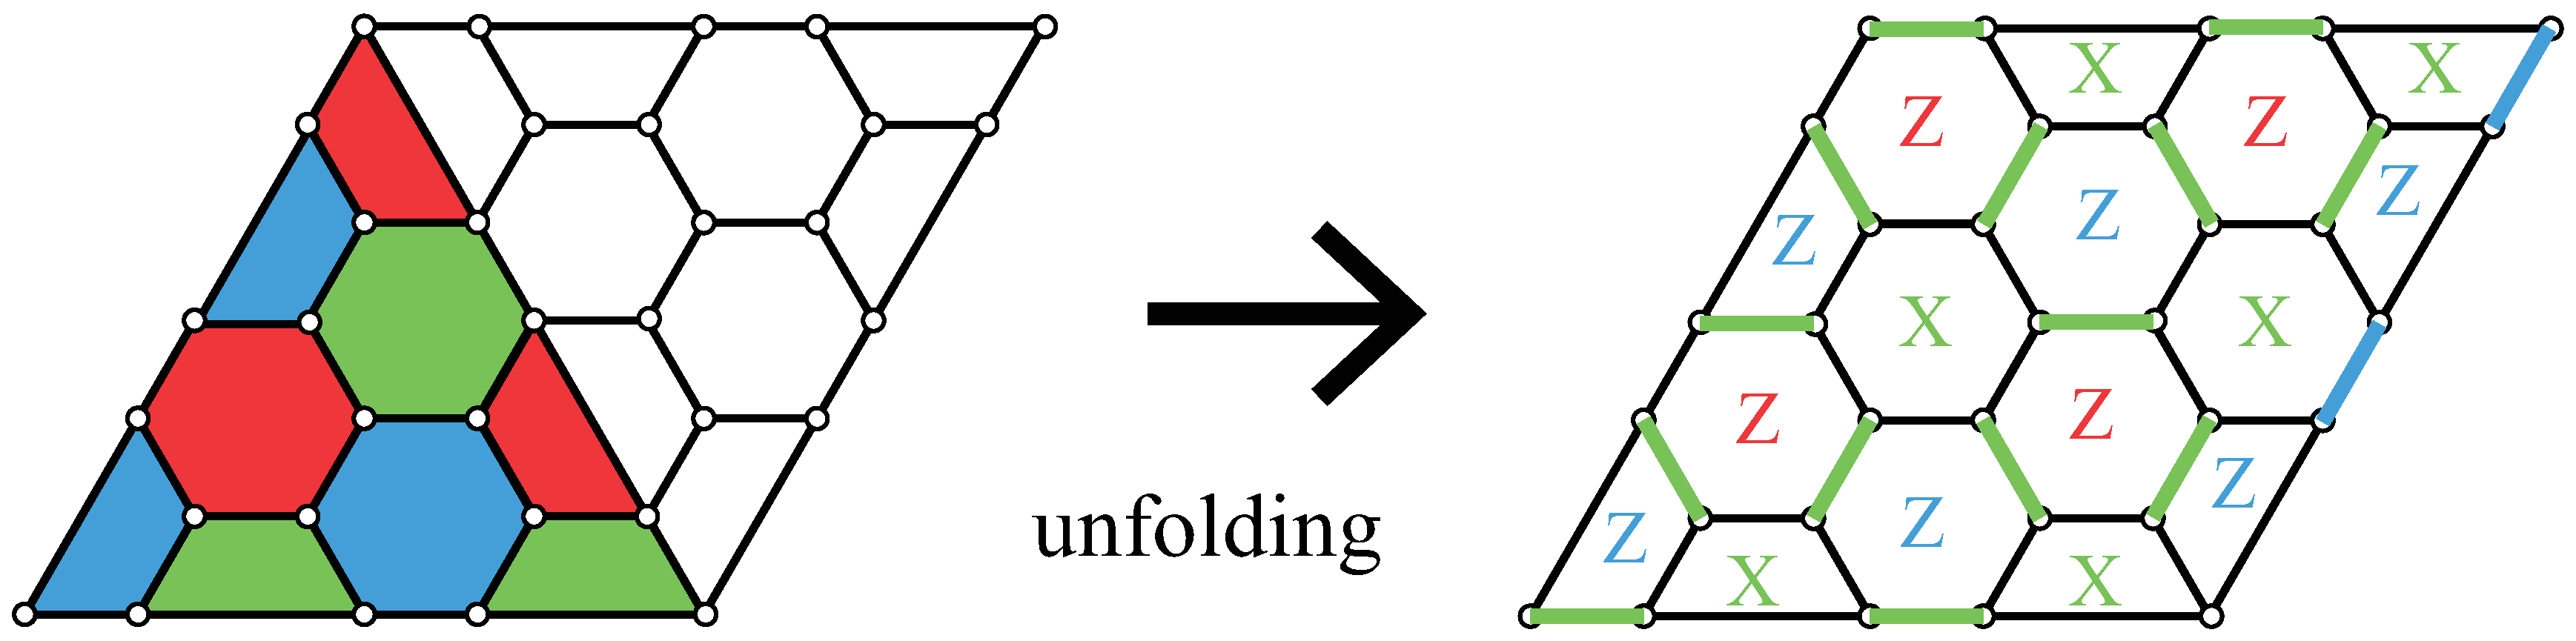
\includegraphics[scale=0.2]{figure/figure1.eps}
        \caption{ }
        \label{figure1}
    \end{figure}

     前回までのunfolding操作をFig.\ref{figure1}に示す。前回の資料(unfolding\_color\_code\_2.pdf)ではあまり折り目の部分について議論しなかったが、よくよく考えてみると折り目の部分の誤り検出は思った以上に難しい。ここではそれを示す。\\
     まず、最初Color Codeから始まったとき、右上部分には$\ket{0}$初期化されているqubitが用意してある。つまり、それらのqubitは1-weight Z stabilizerでスタビライズされている。そのことを、水色をZ stabilizerとしてFig.\ref{figure2}(a)に示す。このとき、折り目だけに注目すると、Fig.\ref{figure2}(b)に示すように、red face Z stabilizerと付近の1-weight Z stabilizerで六角形のZ stabilizerが構成できる。これより、unfolding操作の折り目をまたがる6-weight Z stabilizerによって折り目付近のXエラーを検出できる。

    \begin{figure}[h]
        \centering
        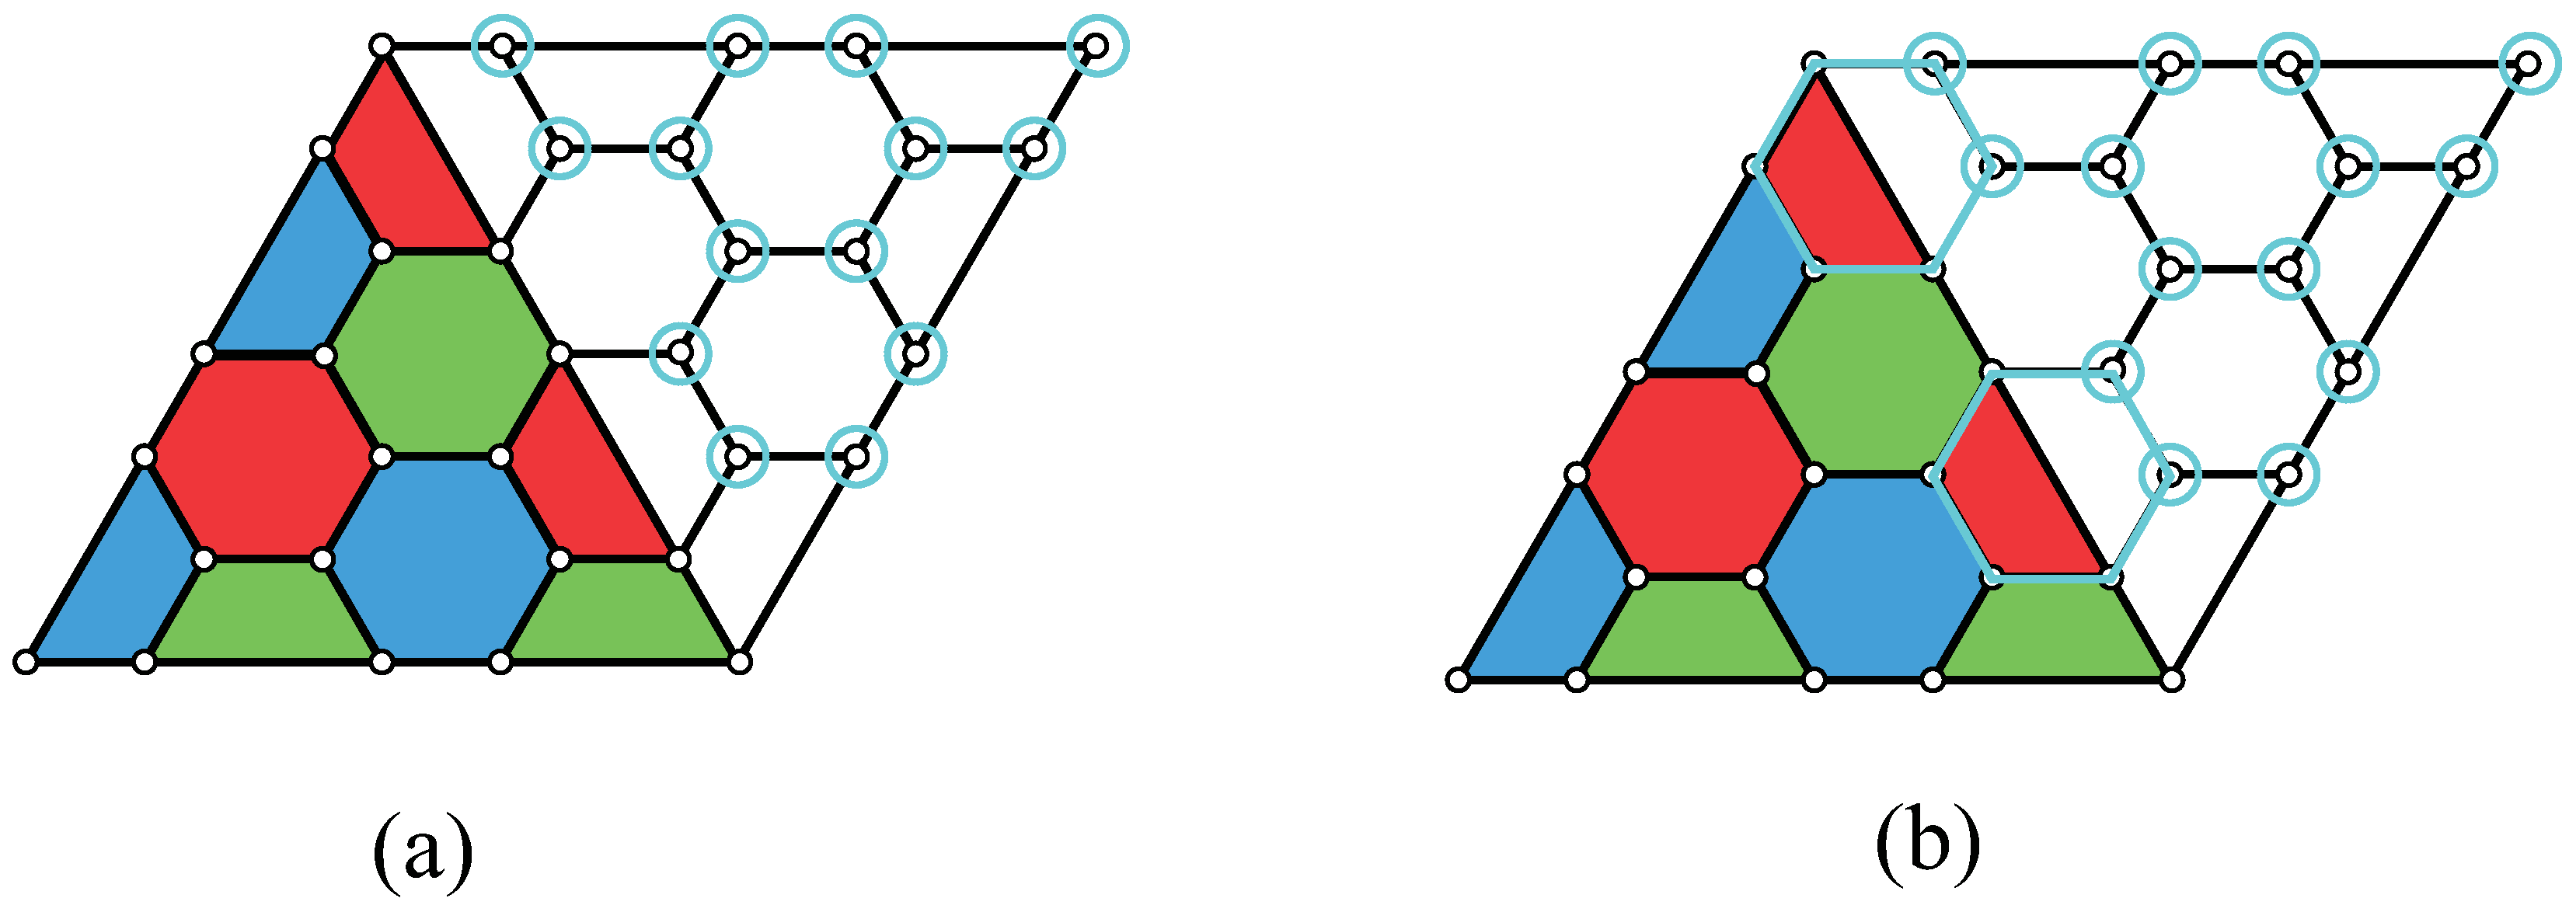
\includegraphics[scale=0.2]{figure/figure2.eps}
        \caption{ }
        \label{figure2}
    \end{figure}

    しかし、Fig.\ref{figure3}に示すような破線の6-weight Z stabilizerはundeterministicである。そのため、Fig.\ref{figure2}(b)の上の水色の六角形のZ stabilizerで検出されたエラーはFig.\ref{figure3}のqubit 1,2,3,4のどこで起きたのかが全くわからない。そのようなことから、前回提示したunfoldingのプロトコルは折り目付近のXエラーが取り除けない。

    \begin{figure}[h]
        \centering
        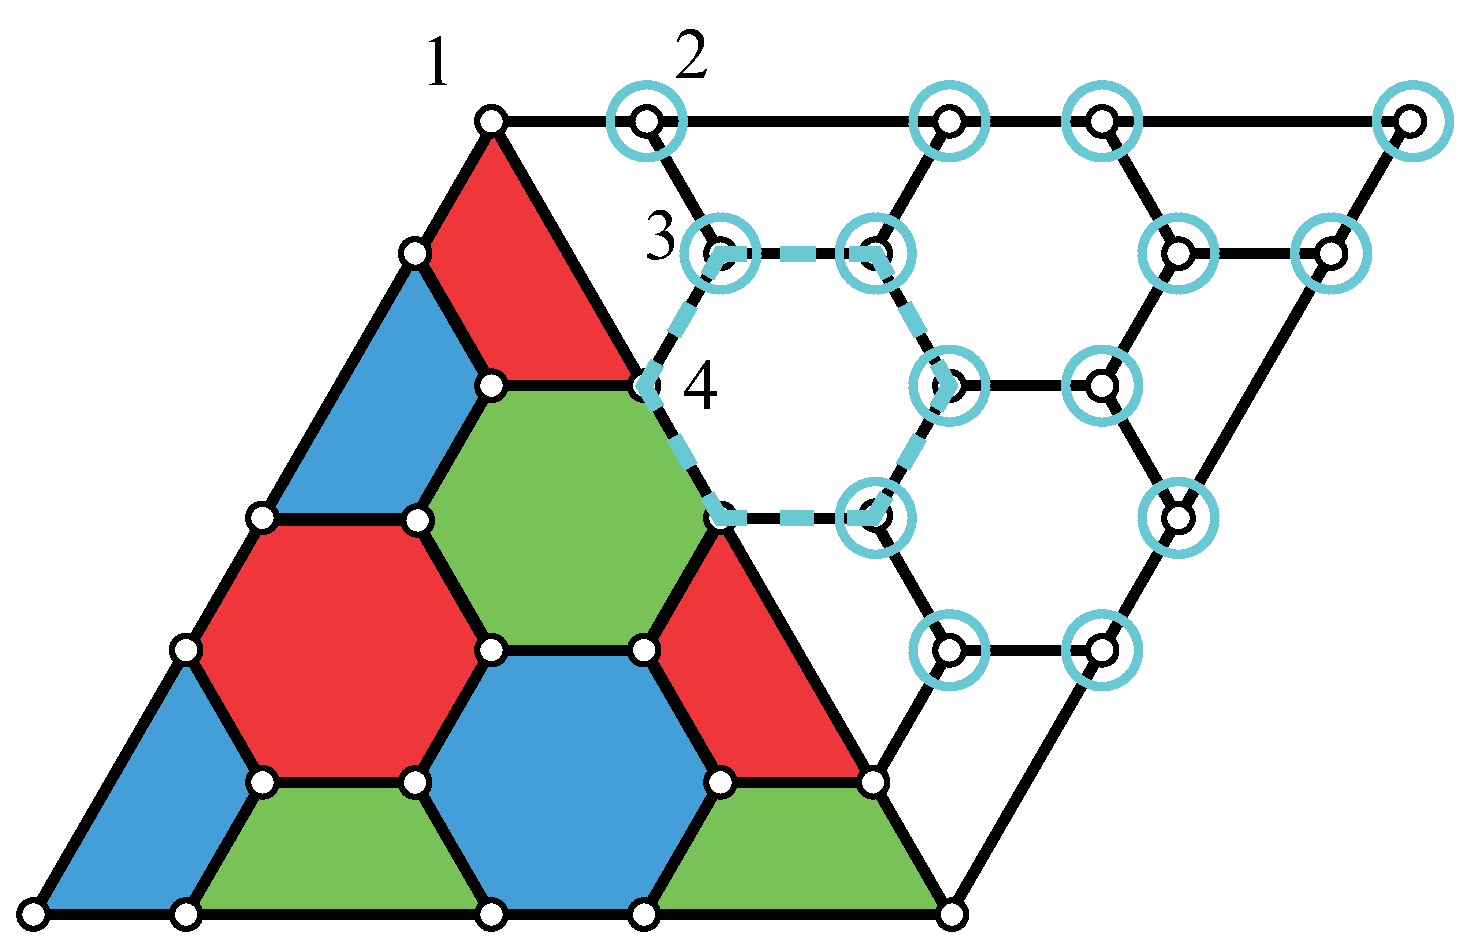
\includegraphics[scale=0.25]{figure/figure3.eps}
        \caption{ }
        \label{figure3}
    \end{figure}

    \clearpage

    また、前回のプロトコルだと折り目付近のZエラーも取り除けないことに気がつく。しかしこれは、折り目付近の2つのqubitをBell 状態にすることによって解決する。それを紫色をX stabilizerとしてFig.\ref{figure4}に示す。ただし、このようにしても上記のXエラーを取り除けない問題は残る。
    
    \begin{figure}[h]
        \centering
        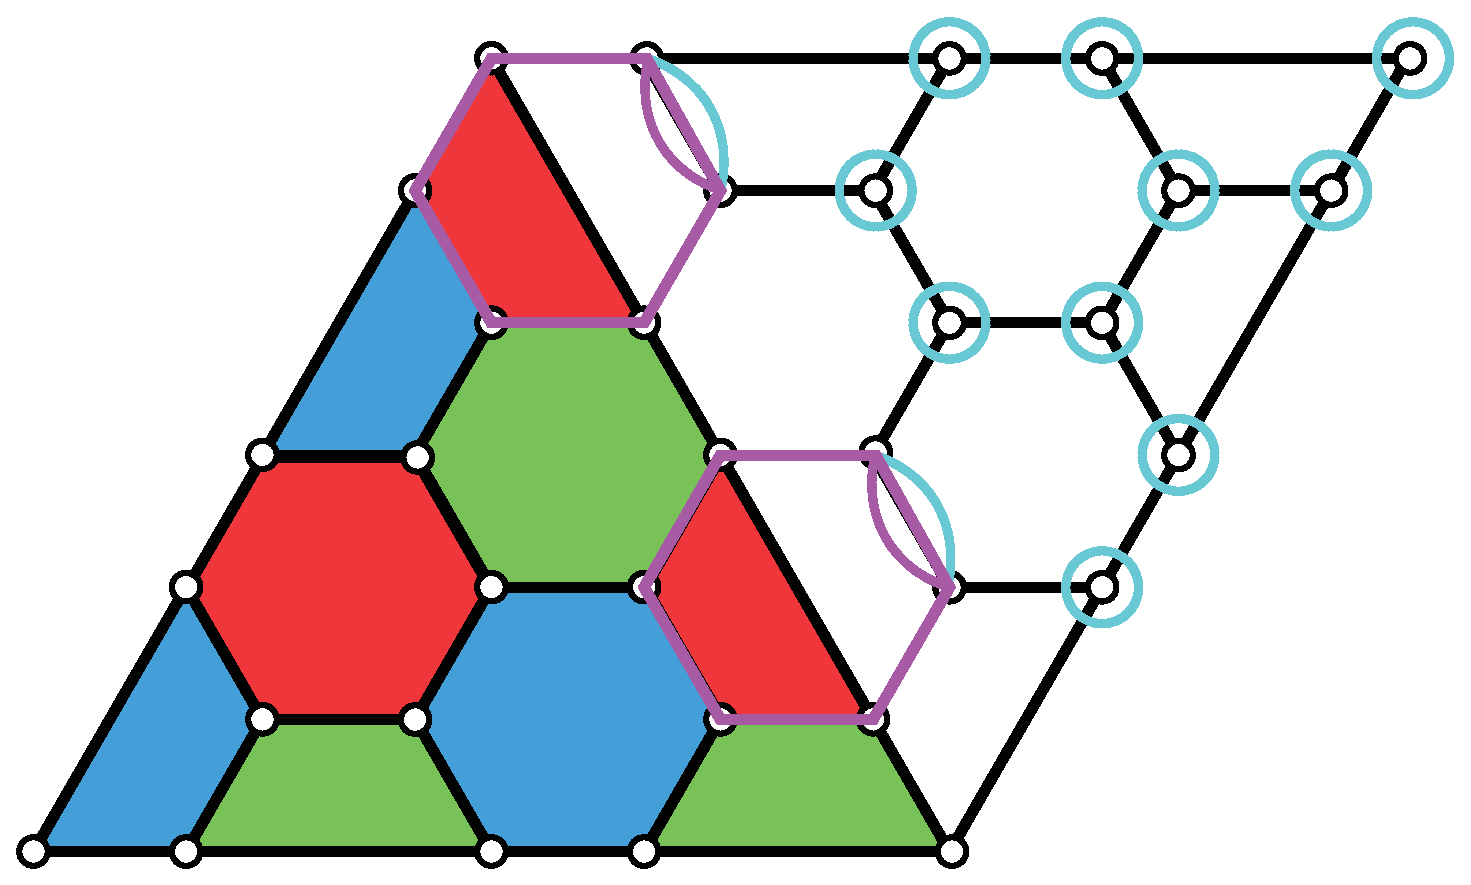
\includegraphics[scale=0.25]{figure/figure4.eps}
        \caption{ }
        \label{figure4}
    \end{figure}

    ということで現状のプロトコルは修正が必要である。参考までにFig.\ref{figure5}に試みた構造の残骸を載せておく。Fig.\ref{figure5}に示すどの構造(stabililzer自体が成り立っていないものもある)をとっても上記と似たような問題が発生した。

    \begin{figure}[h]
        \centering
        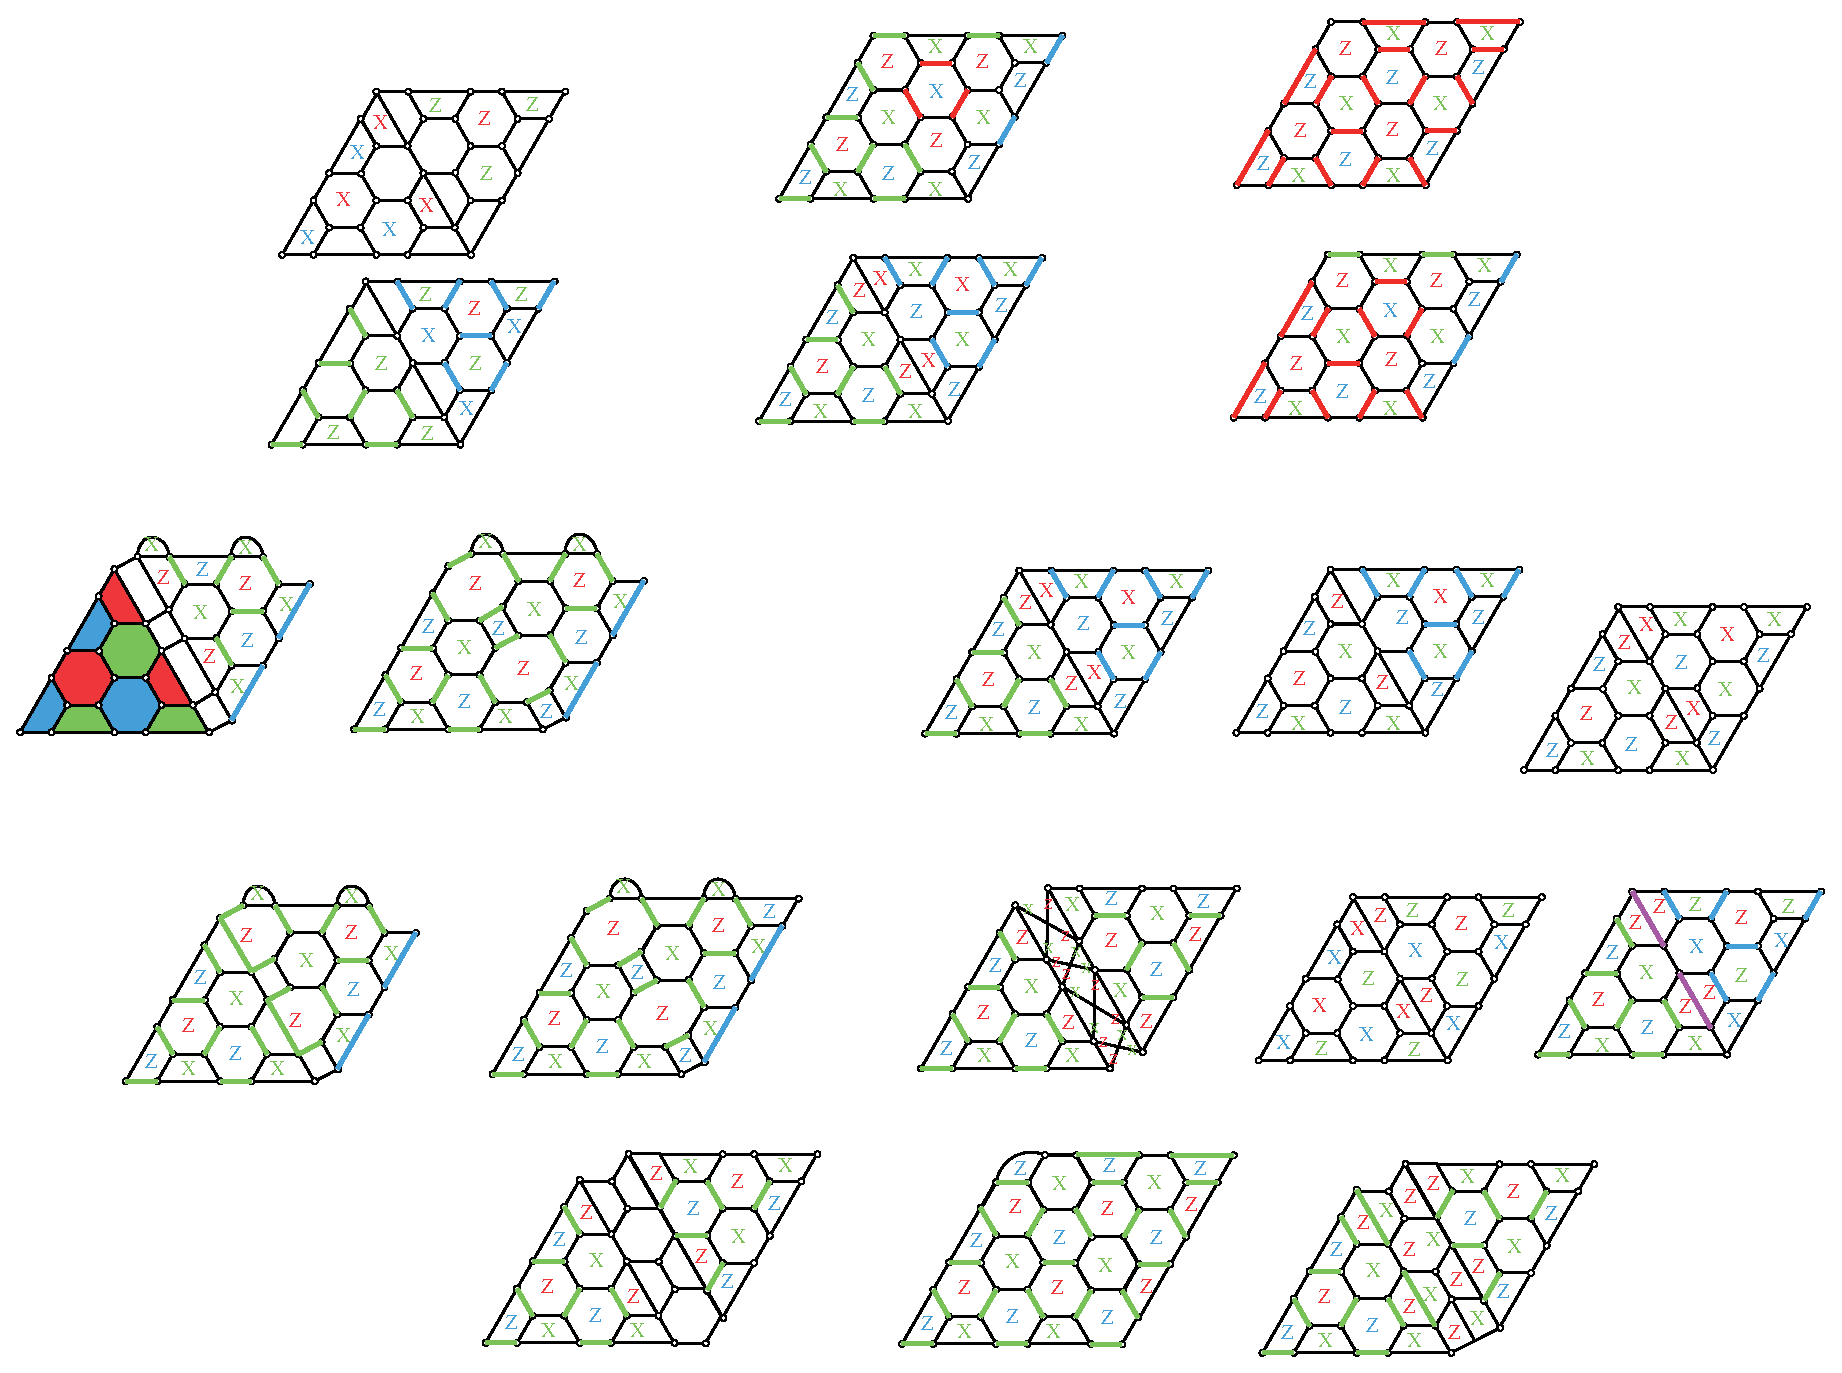
\includegraphics[scale=0.5]{figure/figure5.eps}
        \caption{ }
        \label{figure5}
    \end{figure}
}
\clearpage
 ということで上記の問題の解決策になりそうなものを思いついたのでそれを以下で述べる。
\section{Floquet Code\times Unfolding}\label{floquet_code}{
     Floquet Codeを用いるやり方を思いついたので、まずトーラス上でのFloquet Codeを使ったColor Codeのunfoldingを考える。測定の種類や順番はFig.\ref{figure6}に示す通りである。ここで、Fig.\ref{figure6}にはシンドローム測定するスタビライザーしか示していない。実際にはFig.\ref{figure6}はもっと多くの"示していないスタビライザー"が存在する。

    \begin{figure}[h]
        \centering
        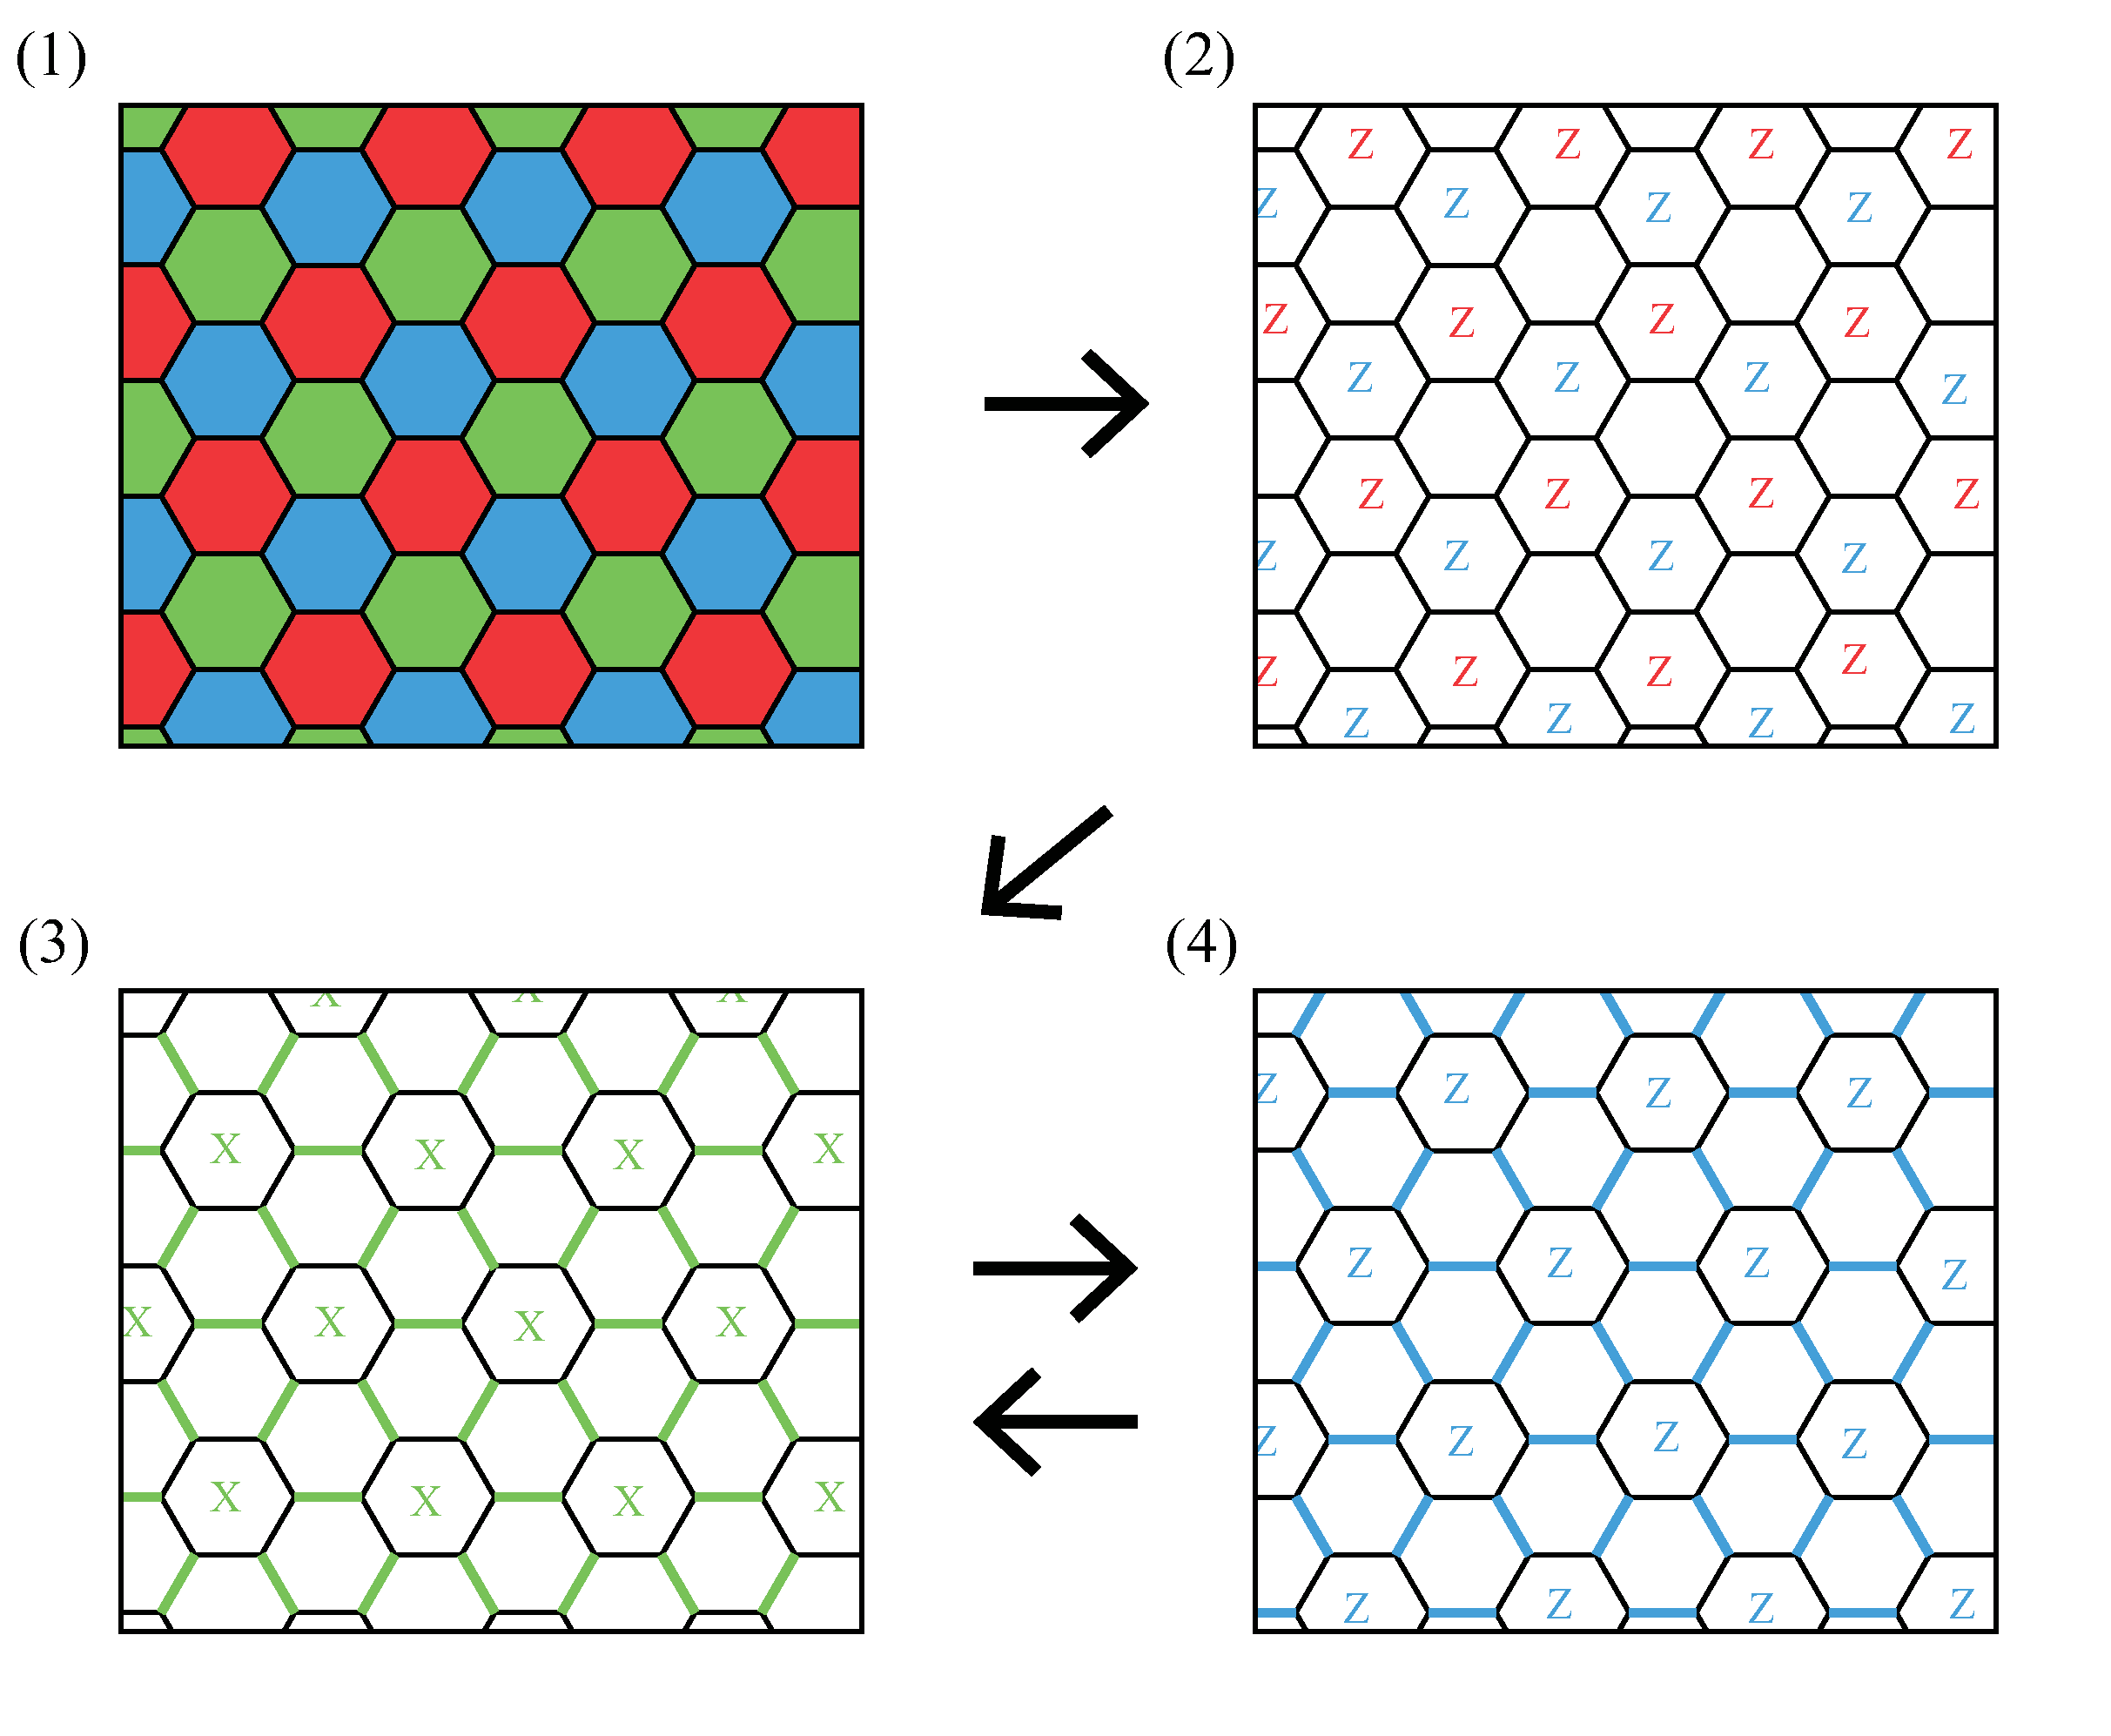
\includegraphics[scale=0.3]{figure/figure6.eps}
        \caption{ }
        \label{figure6}
    \end{figure}

    ここから先、(1),(2),(3),(4)はFig.\ref{figure6}の(1),(2),(3),(4)を表す。まず(1)について、最初はColor CodeなのでそれぞれのfaceにXとZ両方の6-weight stabilizerがある。Z logical operator をgreen edge上に2つ(トーラスの穴をくぐり抜けるものと、穴の周りを一周するもの)取り、X logical operatorをblue edge上に2つ(トーラスの穴をくぐり抜けるものと、穴の周りを一周するもの)取ることとする。その次に(2)でred faceとblue faceについて6-weight Z stabilizerをシンドローム測定すると、 Color Codeのときのシンドローム値と比べることによって、red faceとblue faceに挟まれるedge、つまりgreen edge上のXエラーを検出できる。このとき、green edge上の2つのqubitのうちどちらにXエラーが発生したのかわからないが、どちらかにXゲートをかけて訂正したことにしておく。そして(3)でgreen faceとgreen edge上のスタビライザーでシンドローム測定する。このとき、一個前の(2)で訂正操作が間違っており、Xエラーが発生していない方のqubitにXゲートをかけていた場合の2 qubitエラーはgreen edge上のstabilizerを(3)で導入したことによってスタビライザーそのものとなり、訂正される。また、green faceとred face上の6-weight X stabilizerのシンドローム値(前回の資料と同じようにred faceについてはgreen edge上のスタビライザーをかけ合わせる)がわかるので、blue edge上のZエラーが検出される。これも(2)のときと同じようにblue edge上の2つのqubitのうちどちらにZエラーが発生したのかわからないが、(2)と同じような方法で訂正したこととしておき、(4)でblue faceとblue edge上のスタビライザーを導入することによって、Zエラーは訂正できる。また、(4)での測定によって、(2)と同じred faceとblue face上のZ stabilizerのシンドローム値がわかり、その時に検出されたXエラーは(2)のときと同じように訂正する。以後これを繰り返しエラーを訂正していく。最終的に到達するCodeはSurface Codeそのものである。この一連の操作でgreen edgeとblue edge上のスタビライザーがstabilizer generatorに加えられたり、取り除かれたりされているが、stabilizer generatorの総数は多分変わっていない(簡単に確認しただけで検証はしていない)。また、最初に設定したlogical operatorとはすべて可換な操作なので論理情報は保存されている。
}

\section{Floquet Codeを用いた平面上でのunfolding}{
    ここでは、section \ref{floquet_code}で説明したことを平面で考える。測定の種類や順番はFig.\ref{figure7}に示す通りである。ここで、Fig.\ref{figure7}にはシンドローム測定するスタビライザーしか示していない。実際にはFig.\ref{figure7}はもっと多くの"示していないスタビライザー"が存在する。また、前回の資料(unfolding\_color\_code\_2.pdf)とは色の配置が変わっている。

    \begin{figure}[h]
        \centering
        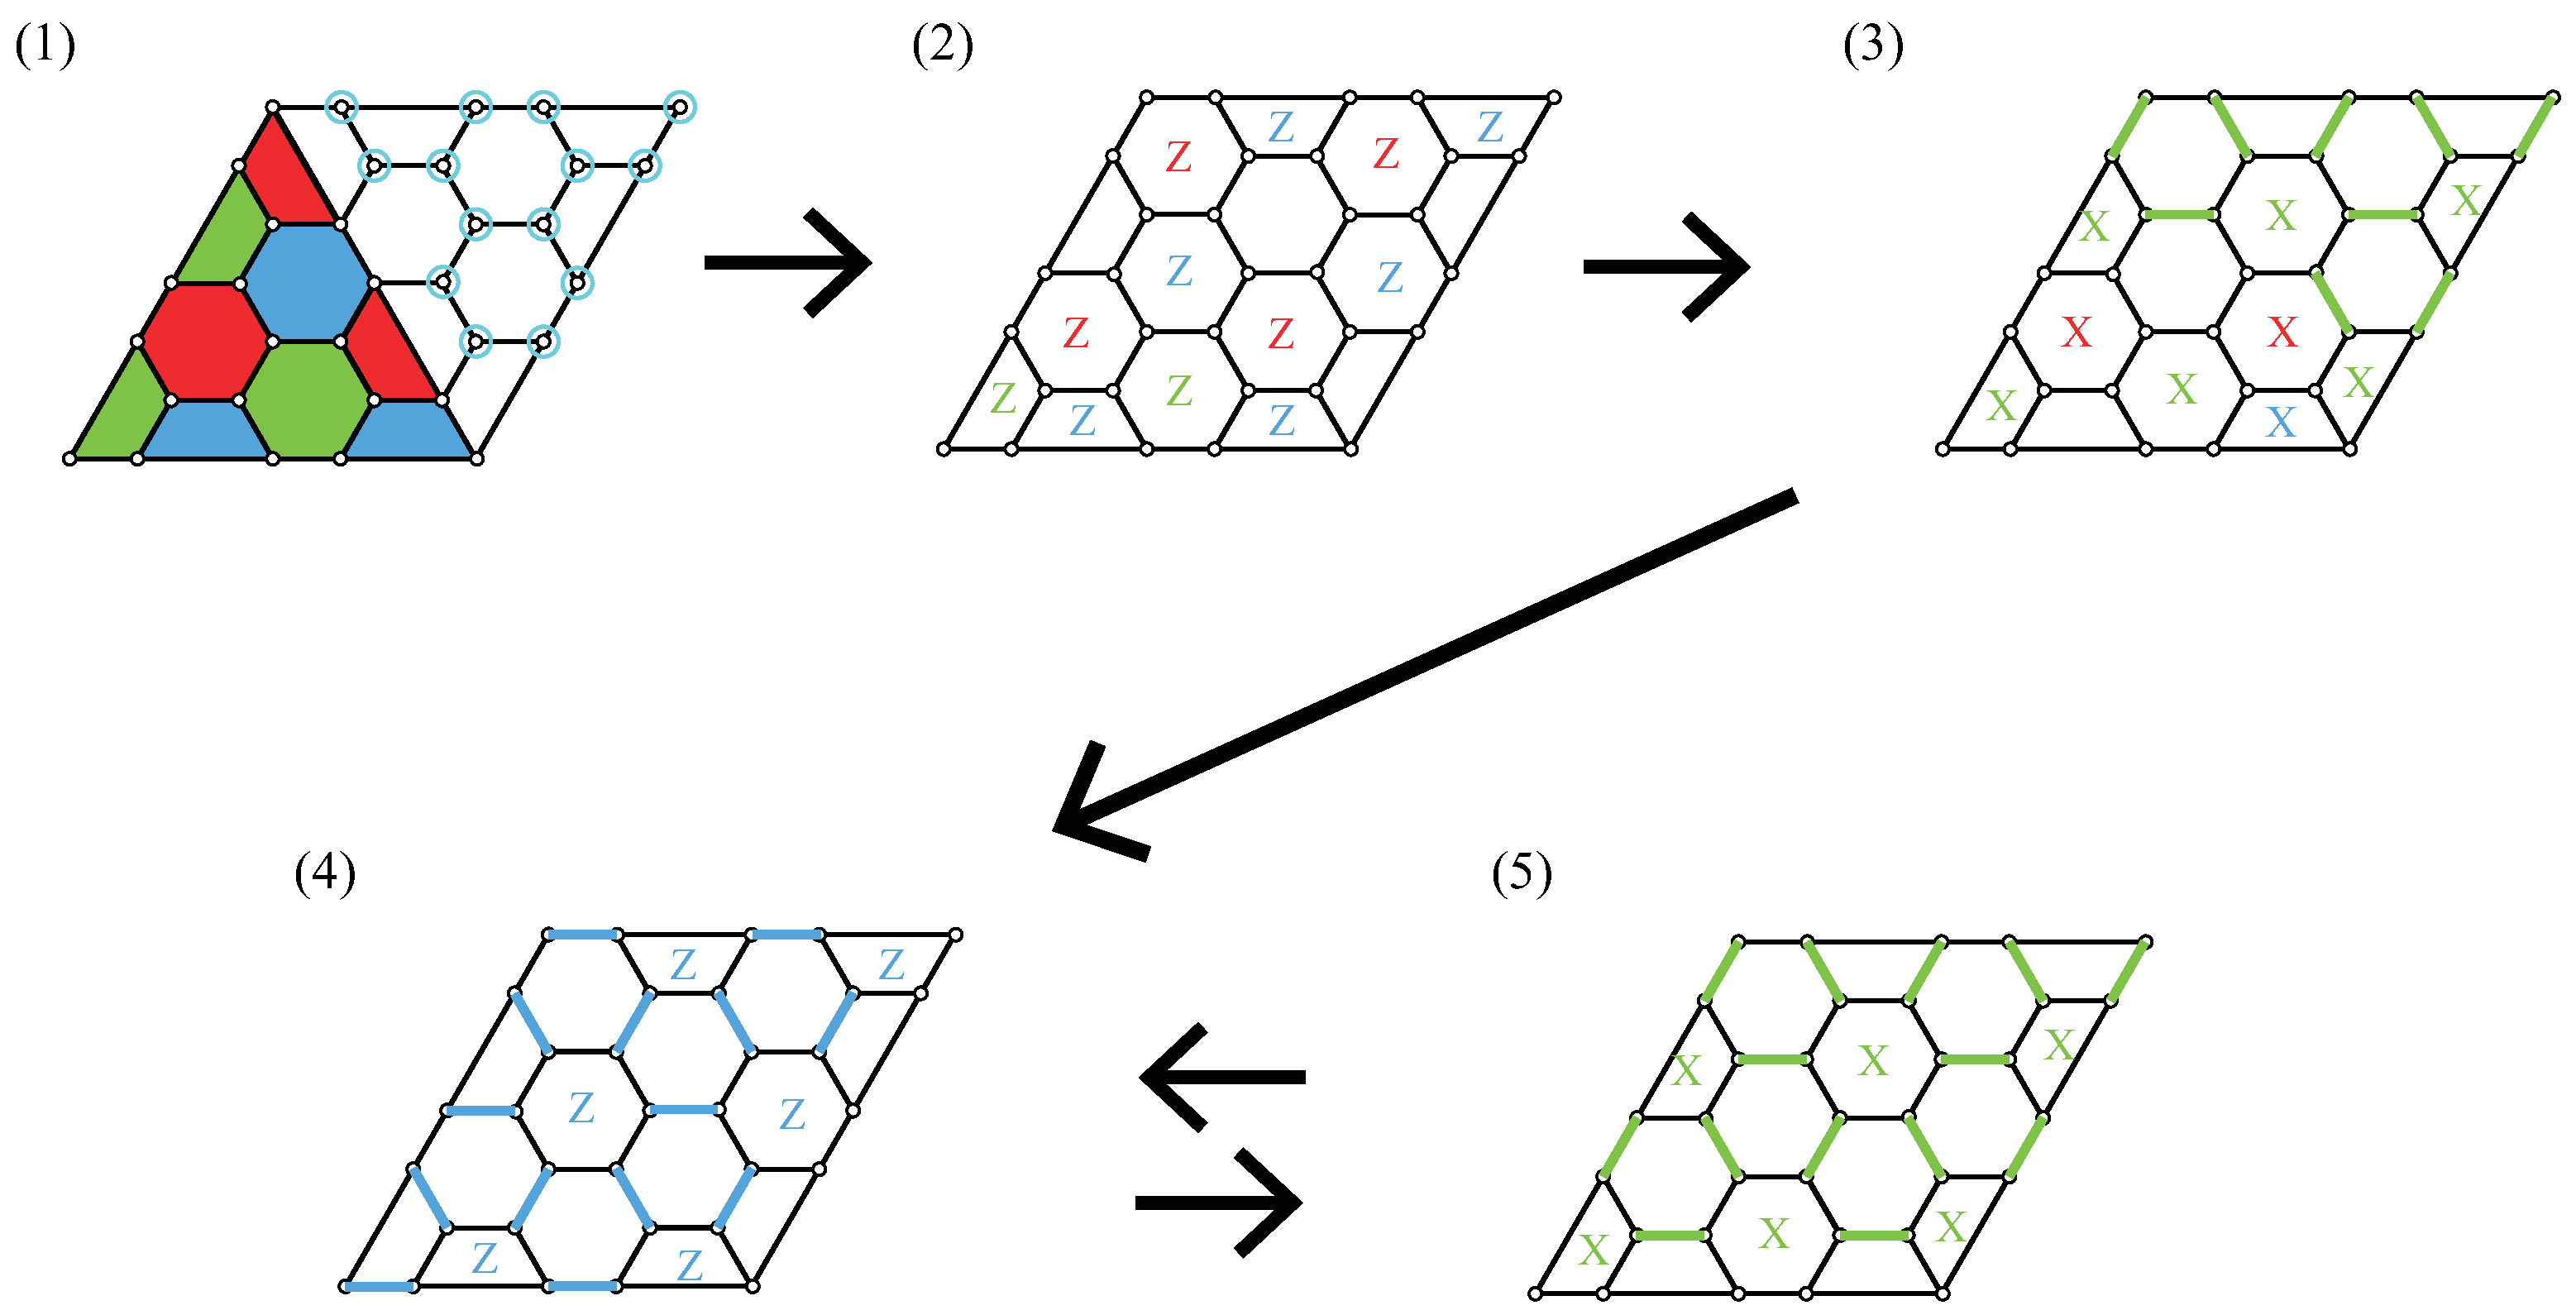
\includegraphics[scale=0.3]{figure/figure7.eps}
        \caption{ }
        \label{figure7}
    \end{figure}

    ここから先、(1),(2),(3),(4),(5)はFig.\ref{figure7}の(1),(2),(3),(4),(5)を表す。具体的な操作やエラー検出、訂正方法はトーラス上で行ったときと同じである。ここでは異なる部分についてのみ説明する。まず、(1)の段階で、Z logical operatorをblue boudaryに取り、X logical operatorをred boudaryに取る。そして、$\ket{0}$初期化されているqubitが右上に用意してある。この段階で、右上で初期化されている領域にもred face、blue faceに対応するZ stabilizerが存在する。次に(2)でシンドローム測定することによってgreen edge上のXエラーは(1)のシンドローム値と比較する事により、拡張した領域も含めて、検出できる。green face上でZ stabilizerを測定している理由はFig.\ref{figure8}に示す通りである。

    \begin{figure}[h]
        \centering
        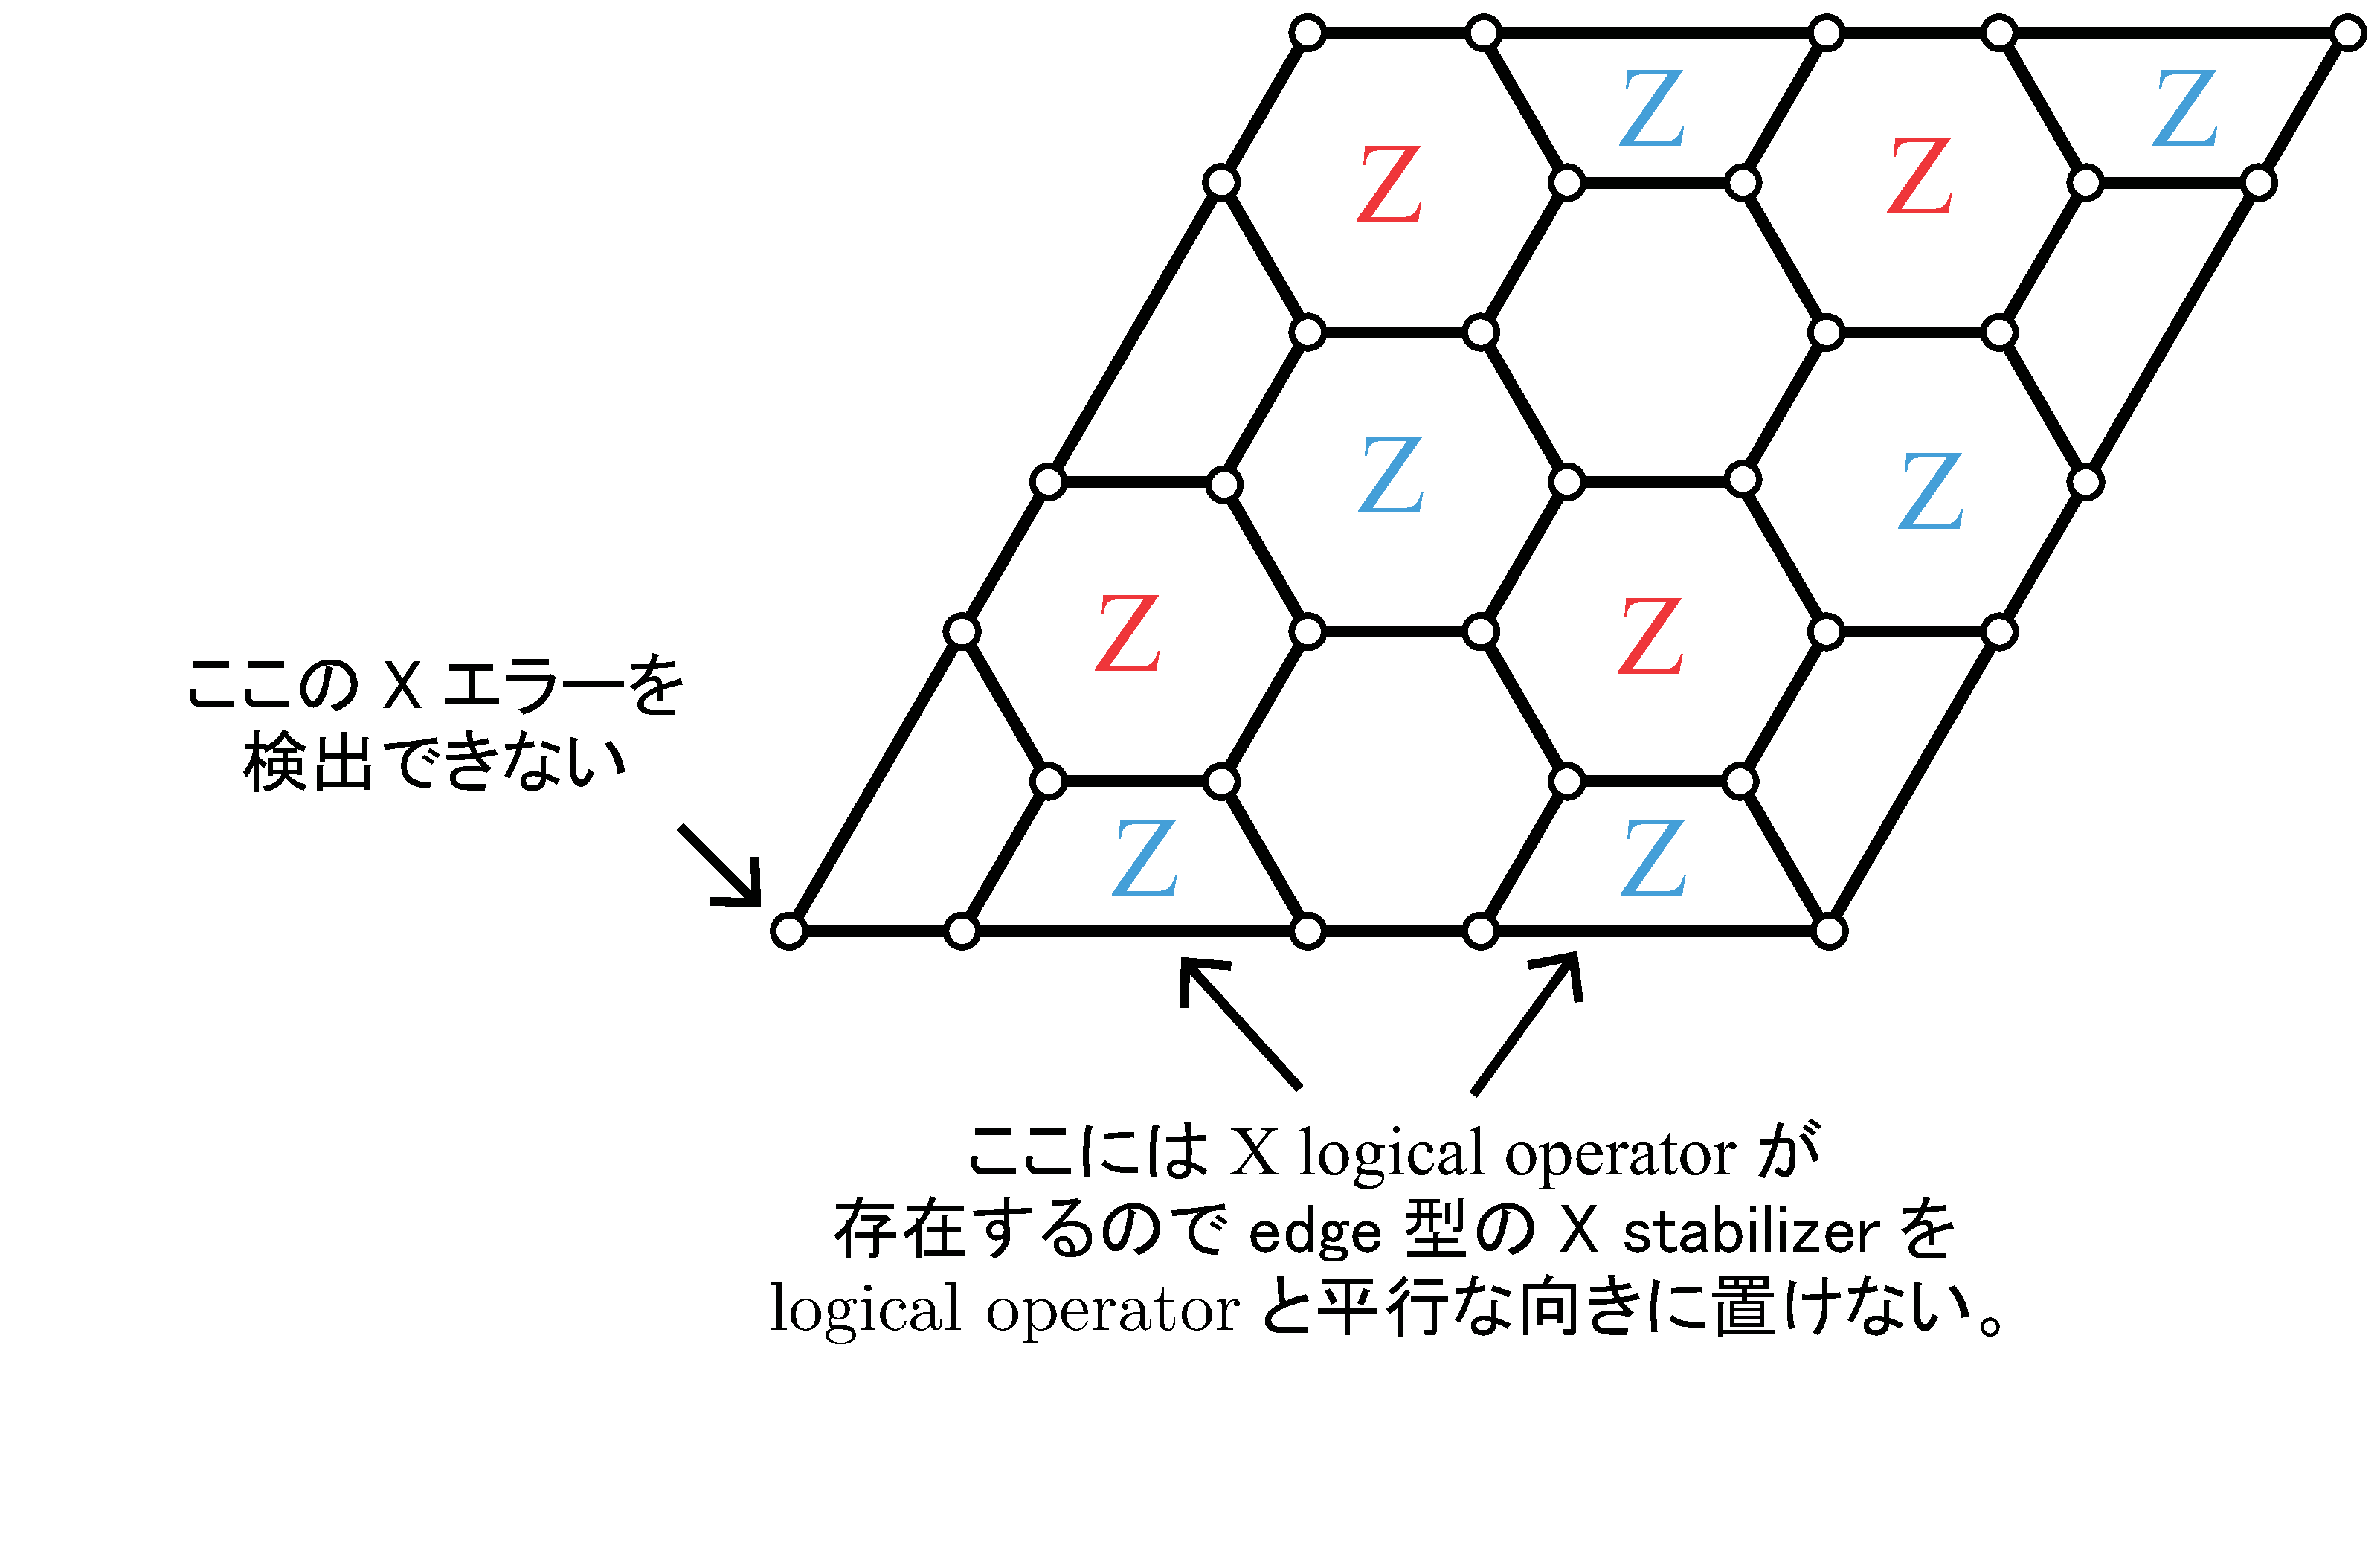
\includegraphics[scale=0.2]{figure/figure8.eps}
        \caption{ }
        \label{figure8}
    \end{figure}

    green face上のZ stabilizerが無いと、まず一番左下のqubitのXエラーが見つけられない、また、一番下のblue face Z stabilizerによって検出されるboudary上のedge(つまり、六角形を半分に切ったときにできるedge)のXエラーはedge上の2 qubitのうちどっちに起こったのかが完全にわからないといけない。なぜなら、そのboundary上にはX logical operatorが存在し、次のステップでそのlogical operatorと平行な方向のedgeにはedge型のstabilizerは置けないからである(logical operatorが縮むから)。そして次に(3)について、右上部分は最初は$\ket{0}$で初期化されているのでZエラーが存在しない。また、blue face X stabilizerが存在するがその理由は(2)の一番左下のqubitに対する議論と同じである。しかしred faceのX stabilizerが存在する理由は(2)とは少し違い、Fig.\ref{figure9}に示すgreen face上のZ stabilizerのシンドローム値を変えたくないからである。幸いなことに一部の左下のgreen edge X stabilizerがなくても、そもそも(2)でそこに存在するXエラーは取り除かれているので問題ない。
    
    \begin{figure}[h]
        \centering
        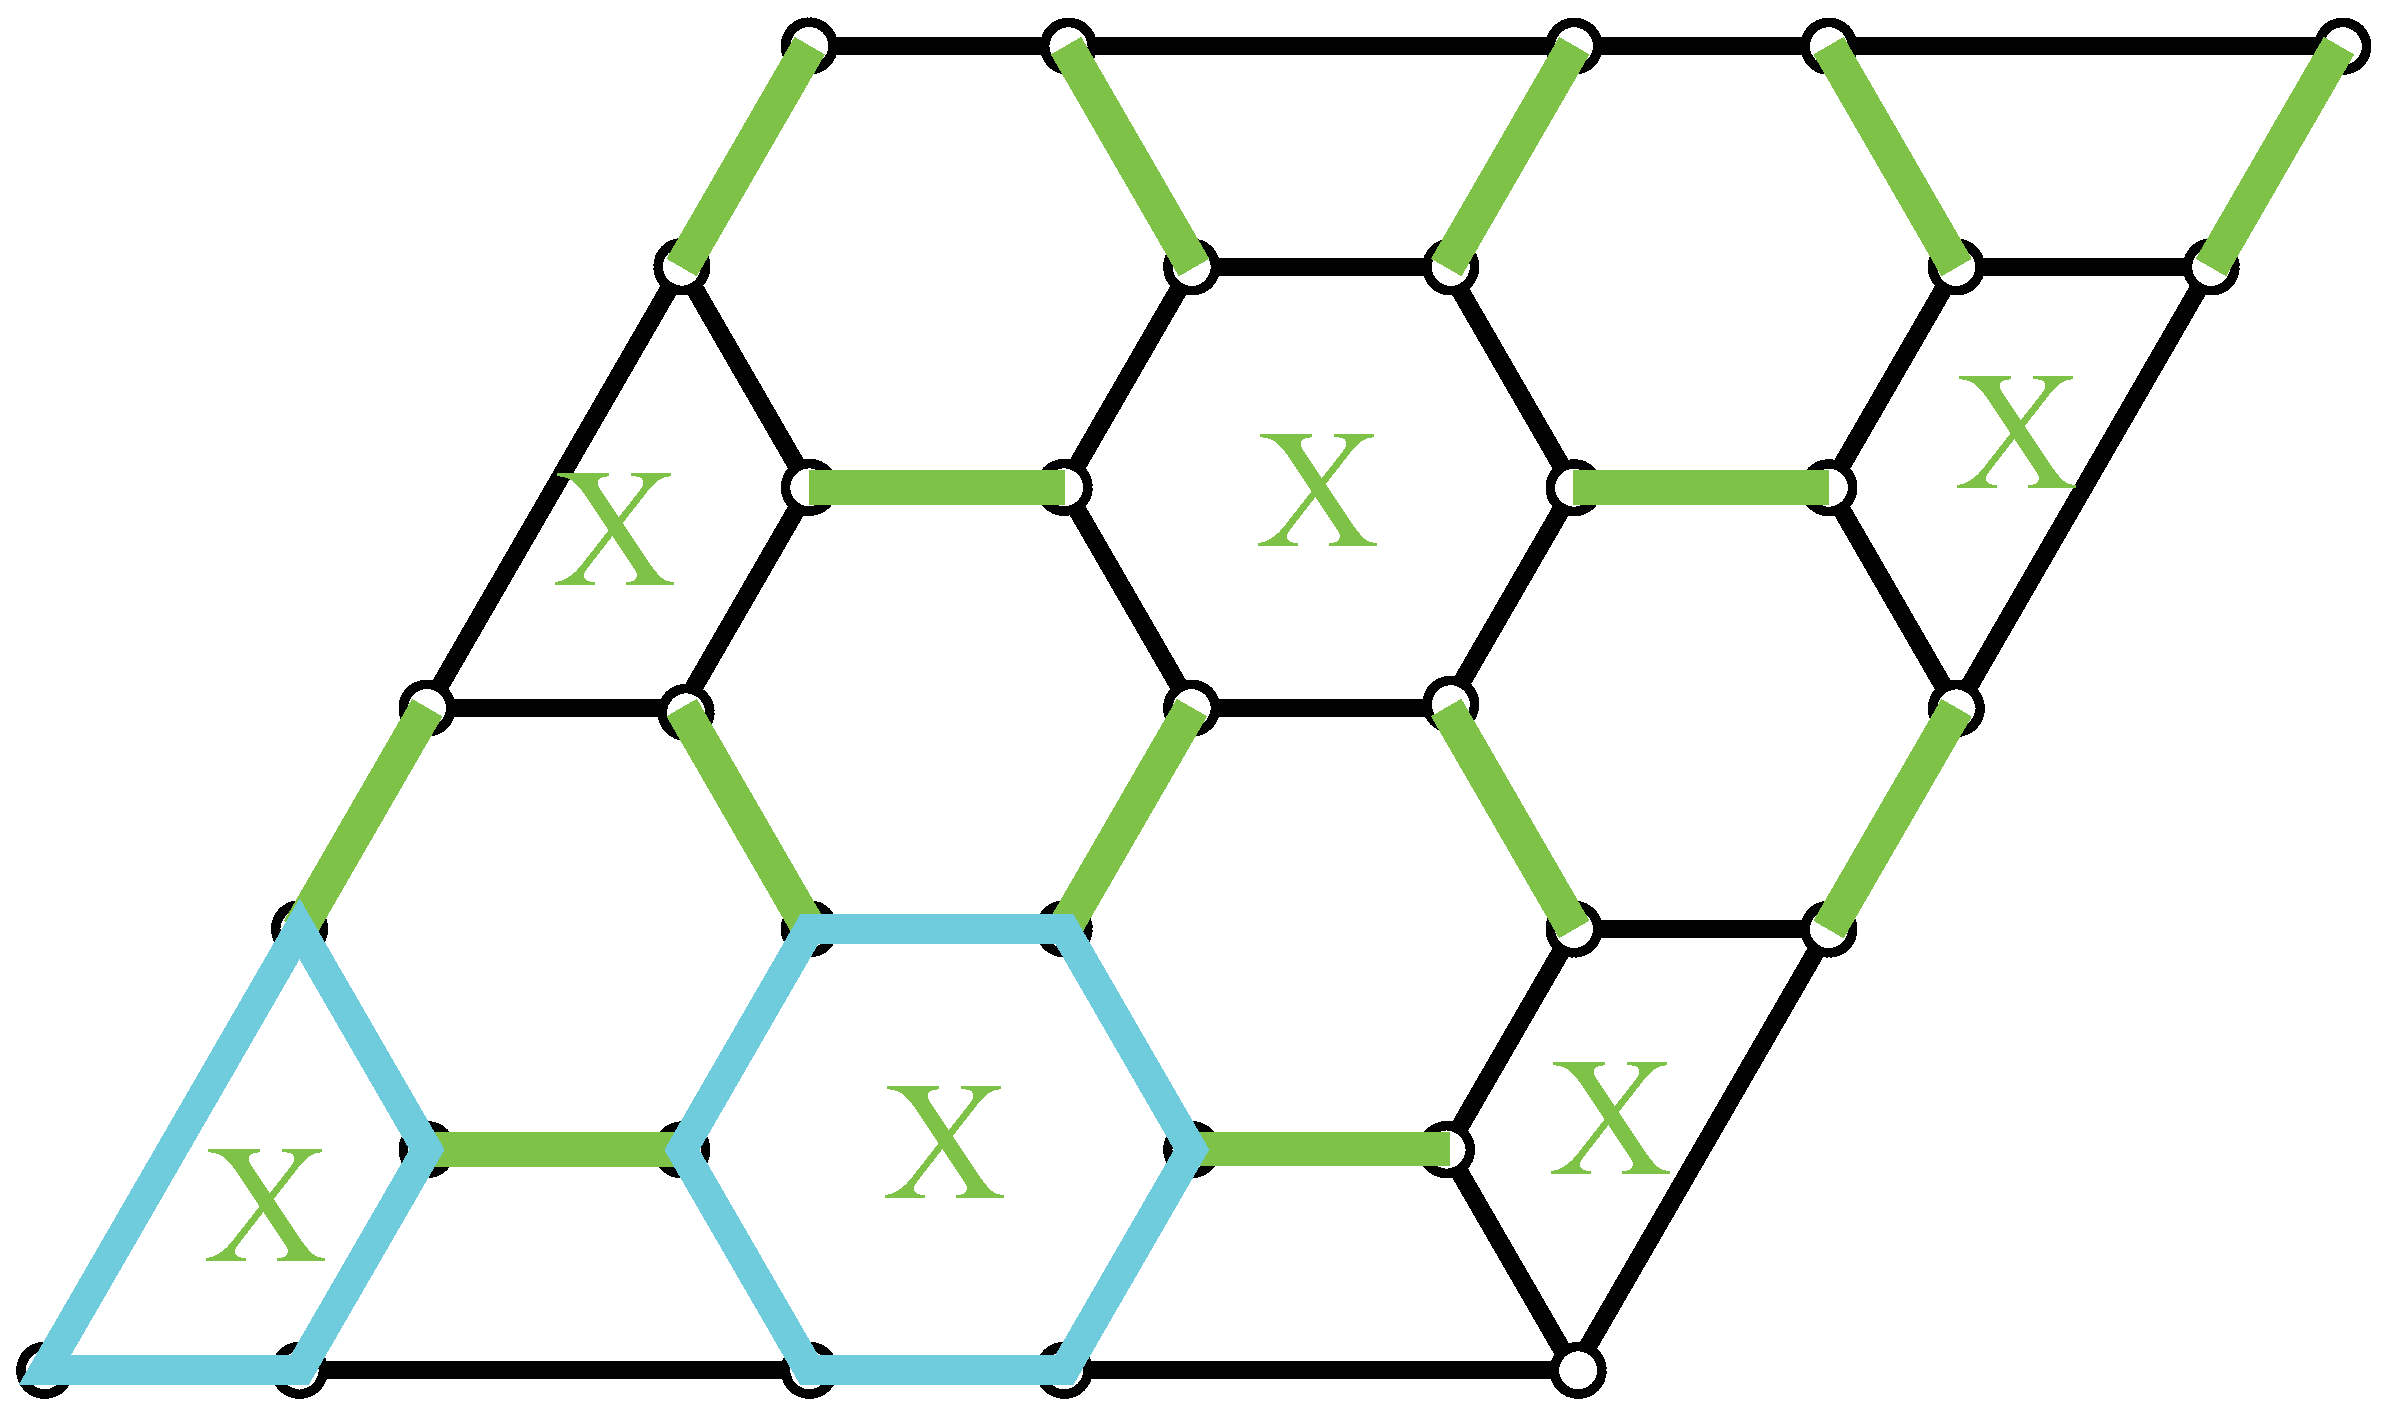
\includegraphics[scale=0.2]{figure/figure9.eps}
        \caption{ }
        \label{figure9}
    \end{figure}

    そして、(4)では、すべてのblue face, red face Z stabilizerのシンドローム値と(3)で守った一部のgreen faceのZ stabilizerのシンドローム値が確定しているのですべてのXエラーを取り除ける。そして(5)では全てのgreen face,red face X stabilizerのシンドローム値は確定しているのですべてのZエラーが取り除ける。周期1回目が終わったあとは平行四辺形の下と右にそれぞれedge型のZ stabilizerとX stabilizerが常に存在するようになるので、下と右のboundary上はedge stabilizerのシンドローム値をそのまま用いてエラー検出を行う。\\
     ということで最終的なスタビライザーをすべて示した図をFig.\ref{figure10}に示しておく。

    \begin{figure}[h]
        \centering
        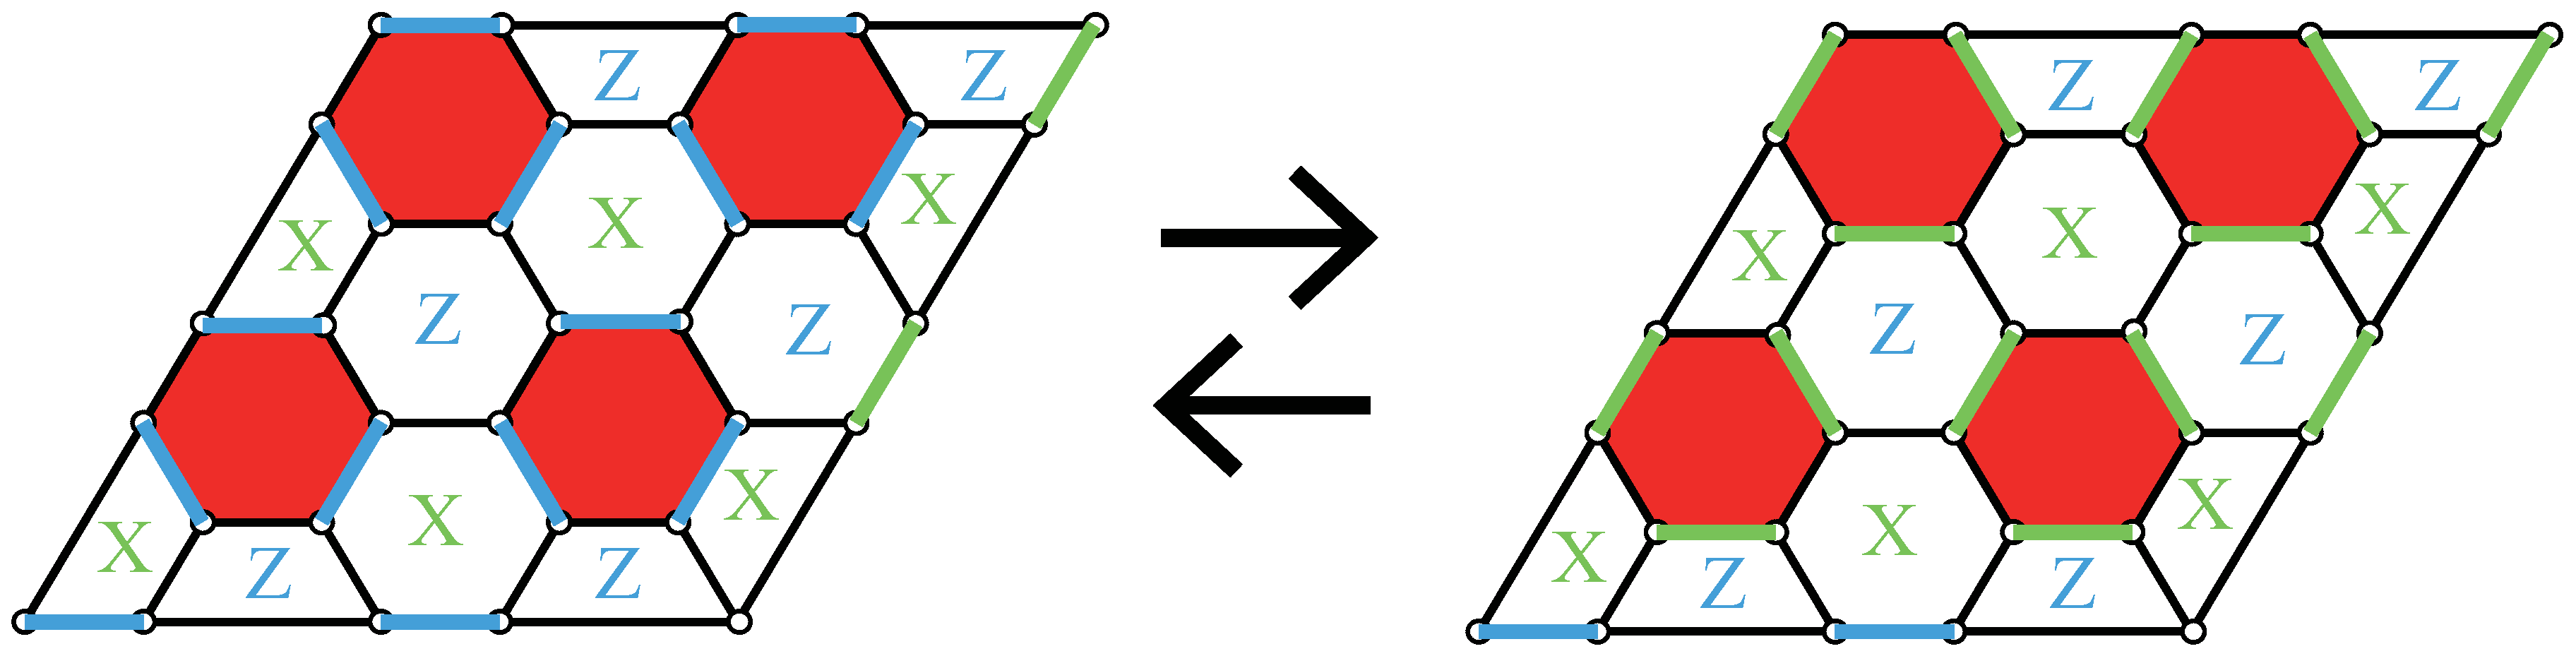
\includegraphics[scale=0.25]{figure/figure10.eps}
        \caption{ }
        \label{figure10}
    \end{figure}
}
\clearpage

\section{CNOTの順序}{

    \begin{figure}[h]
        \centering
        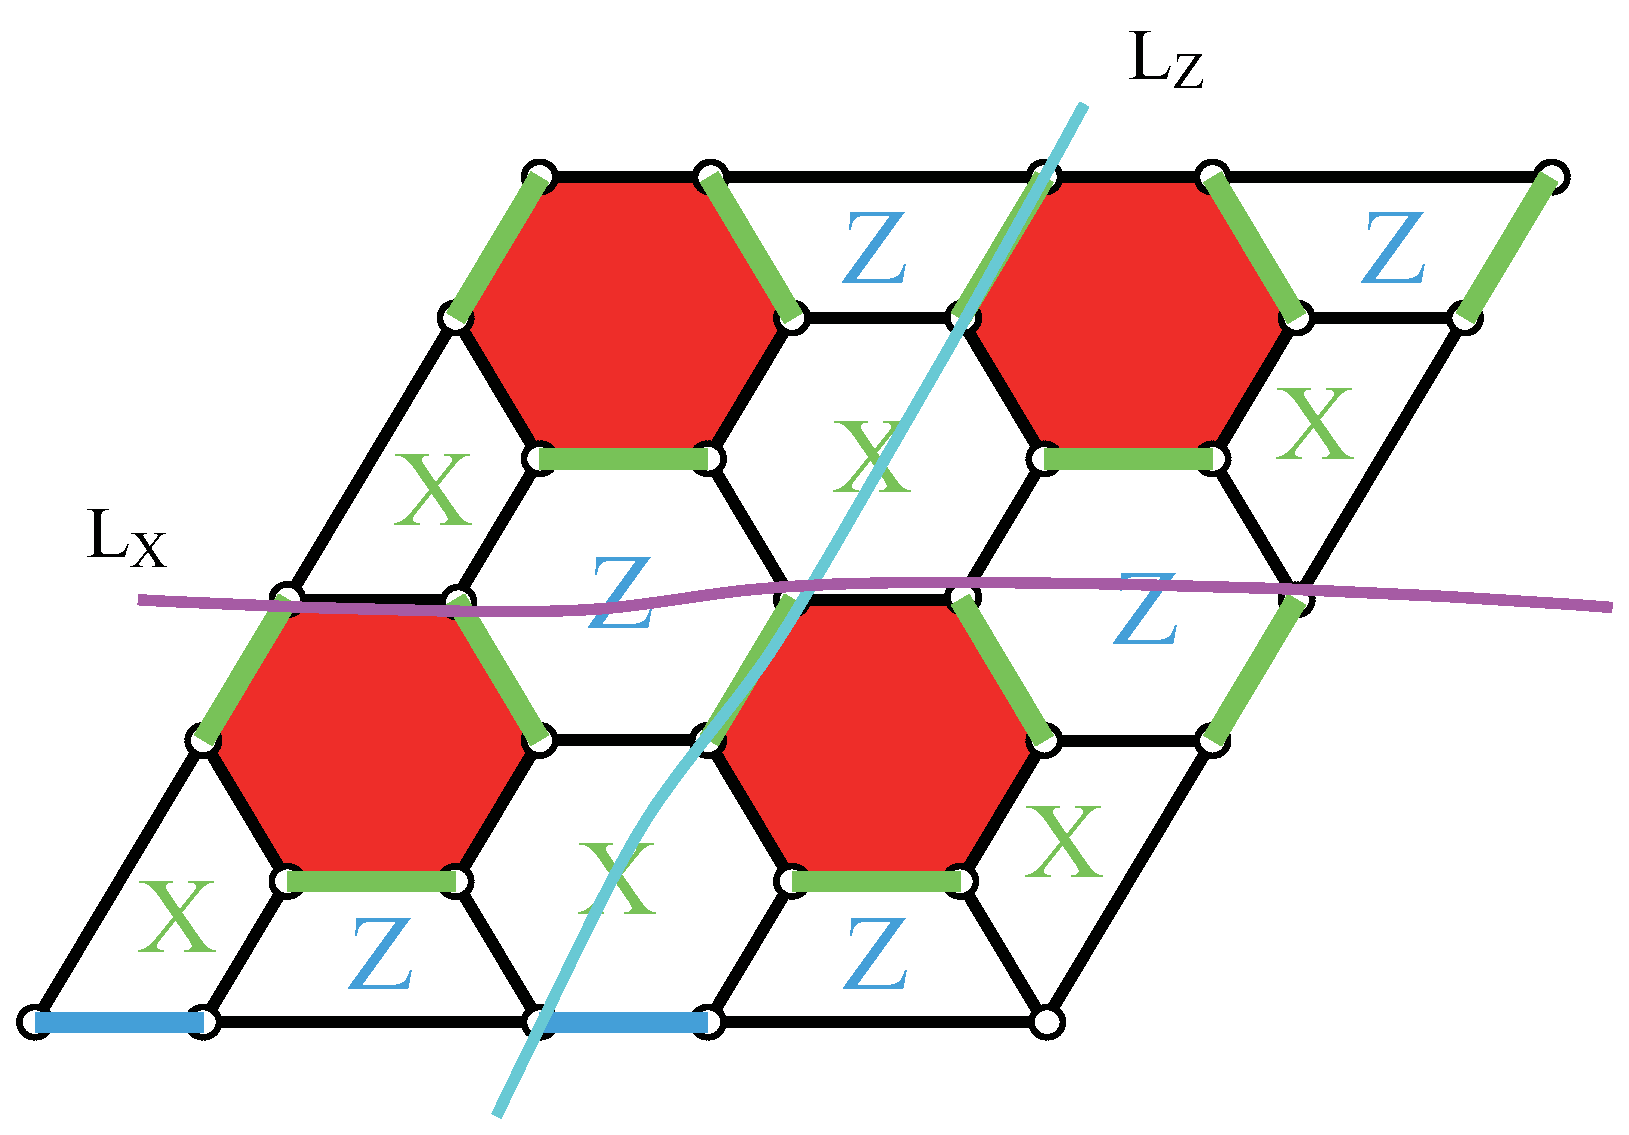
\includegraphics[scale=0.25]{figure/figure11.eps}
        \caption{ }
        \label{figure11}
    \end{figure}

    また、エラー伝播により実効的なcode distanceが小さくなるのを防ぐこともできそうである。基本的に正方形を敷き詰めて作るsurface codeと考え方は同じである。Fig.\ref{figure11}でいうと、6-weightの多体pauli測定をする際にancilla qubitからのエラーについて、水平方向にXエラーが、水平から$60^\circ$の方向にZエラーが蓄積しなければいい。それを満たす手順とエラー伝播の種類をFig.\ref{figure12}に示す。

    \begin{figure}[h]
        \centering
        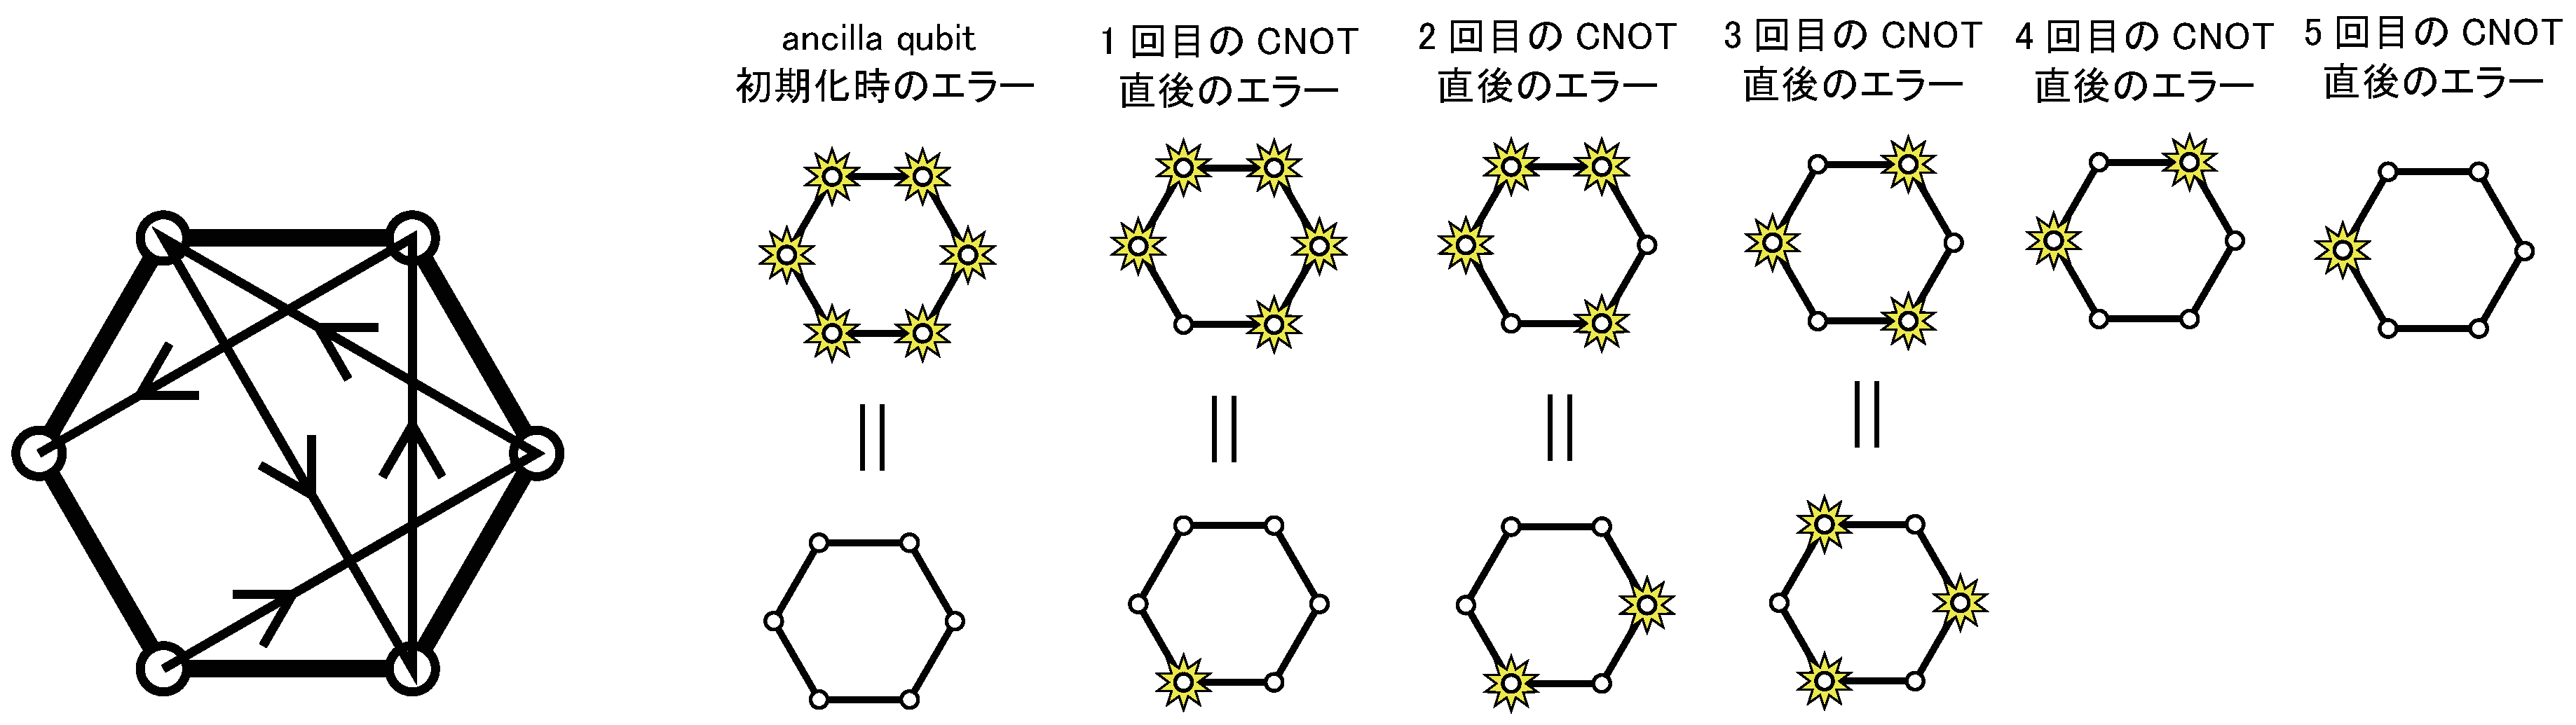
\includegraphics[scale=0.25]{figure/figure12.eps}
        \caption{ }
        \label{figure12}
    \end{figure}

    Fig.\ref{figure12}から、水平方向、水平から$60^\circ$方向のどちらにも2つのエラーが伝搬していないから、X,Z stabilizerの両方をこのCNOT順序で実行すれば良い。
}
\clearpage

\section{拡大}{
     最後にunfolding操作と同時に拡大する手順を載せておく(Fig.\ref{figure13})。正方形Surface Codeの領域はオレンジがX stabilizerで青色がZ stabilizerである。

    \begin{figure}[h]
        \centering
        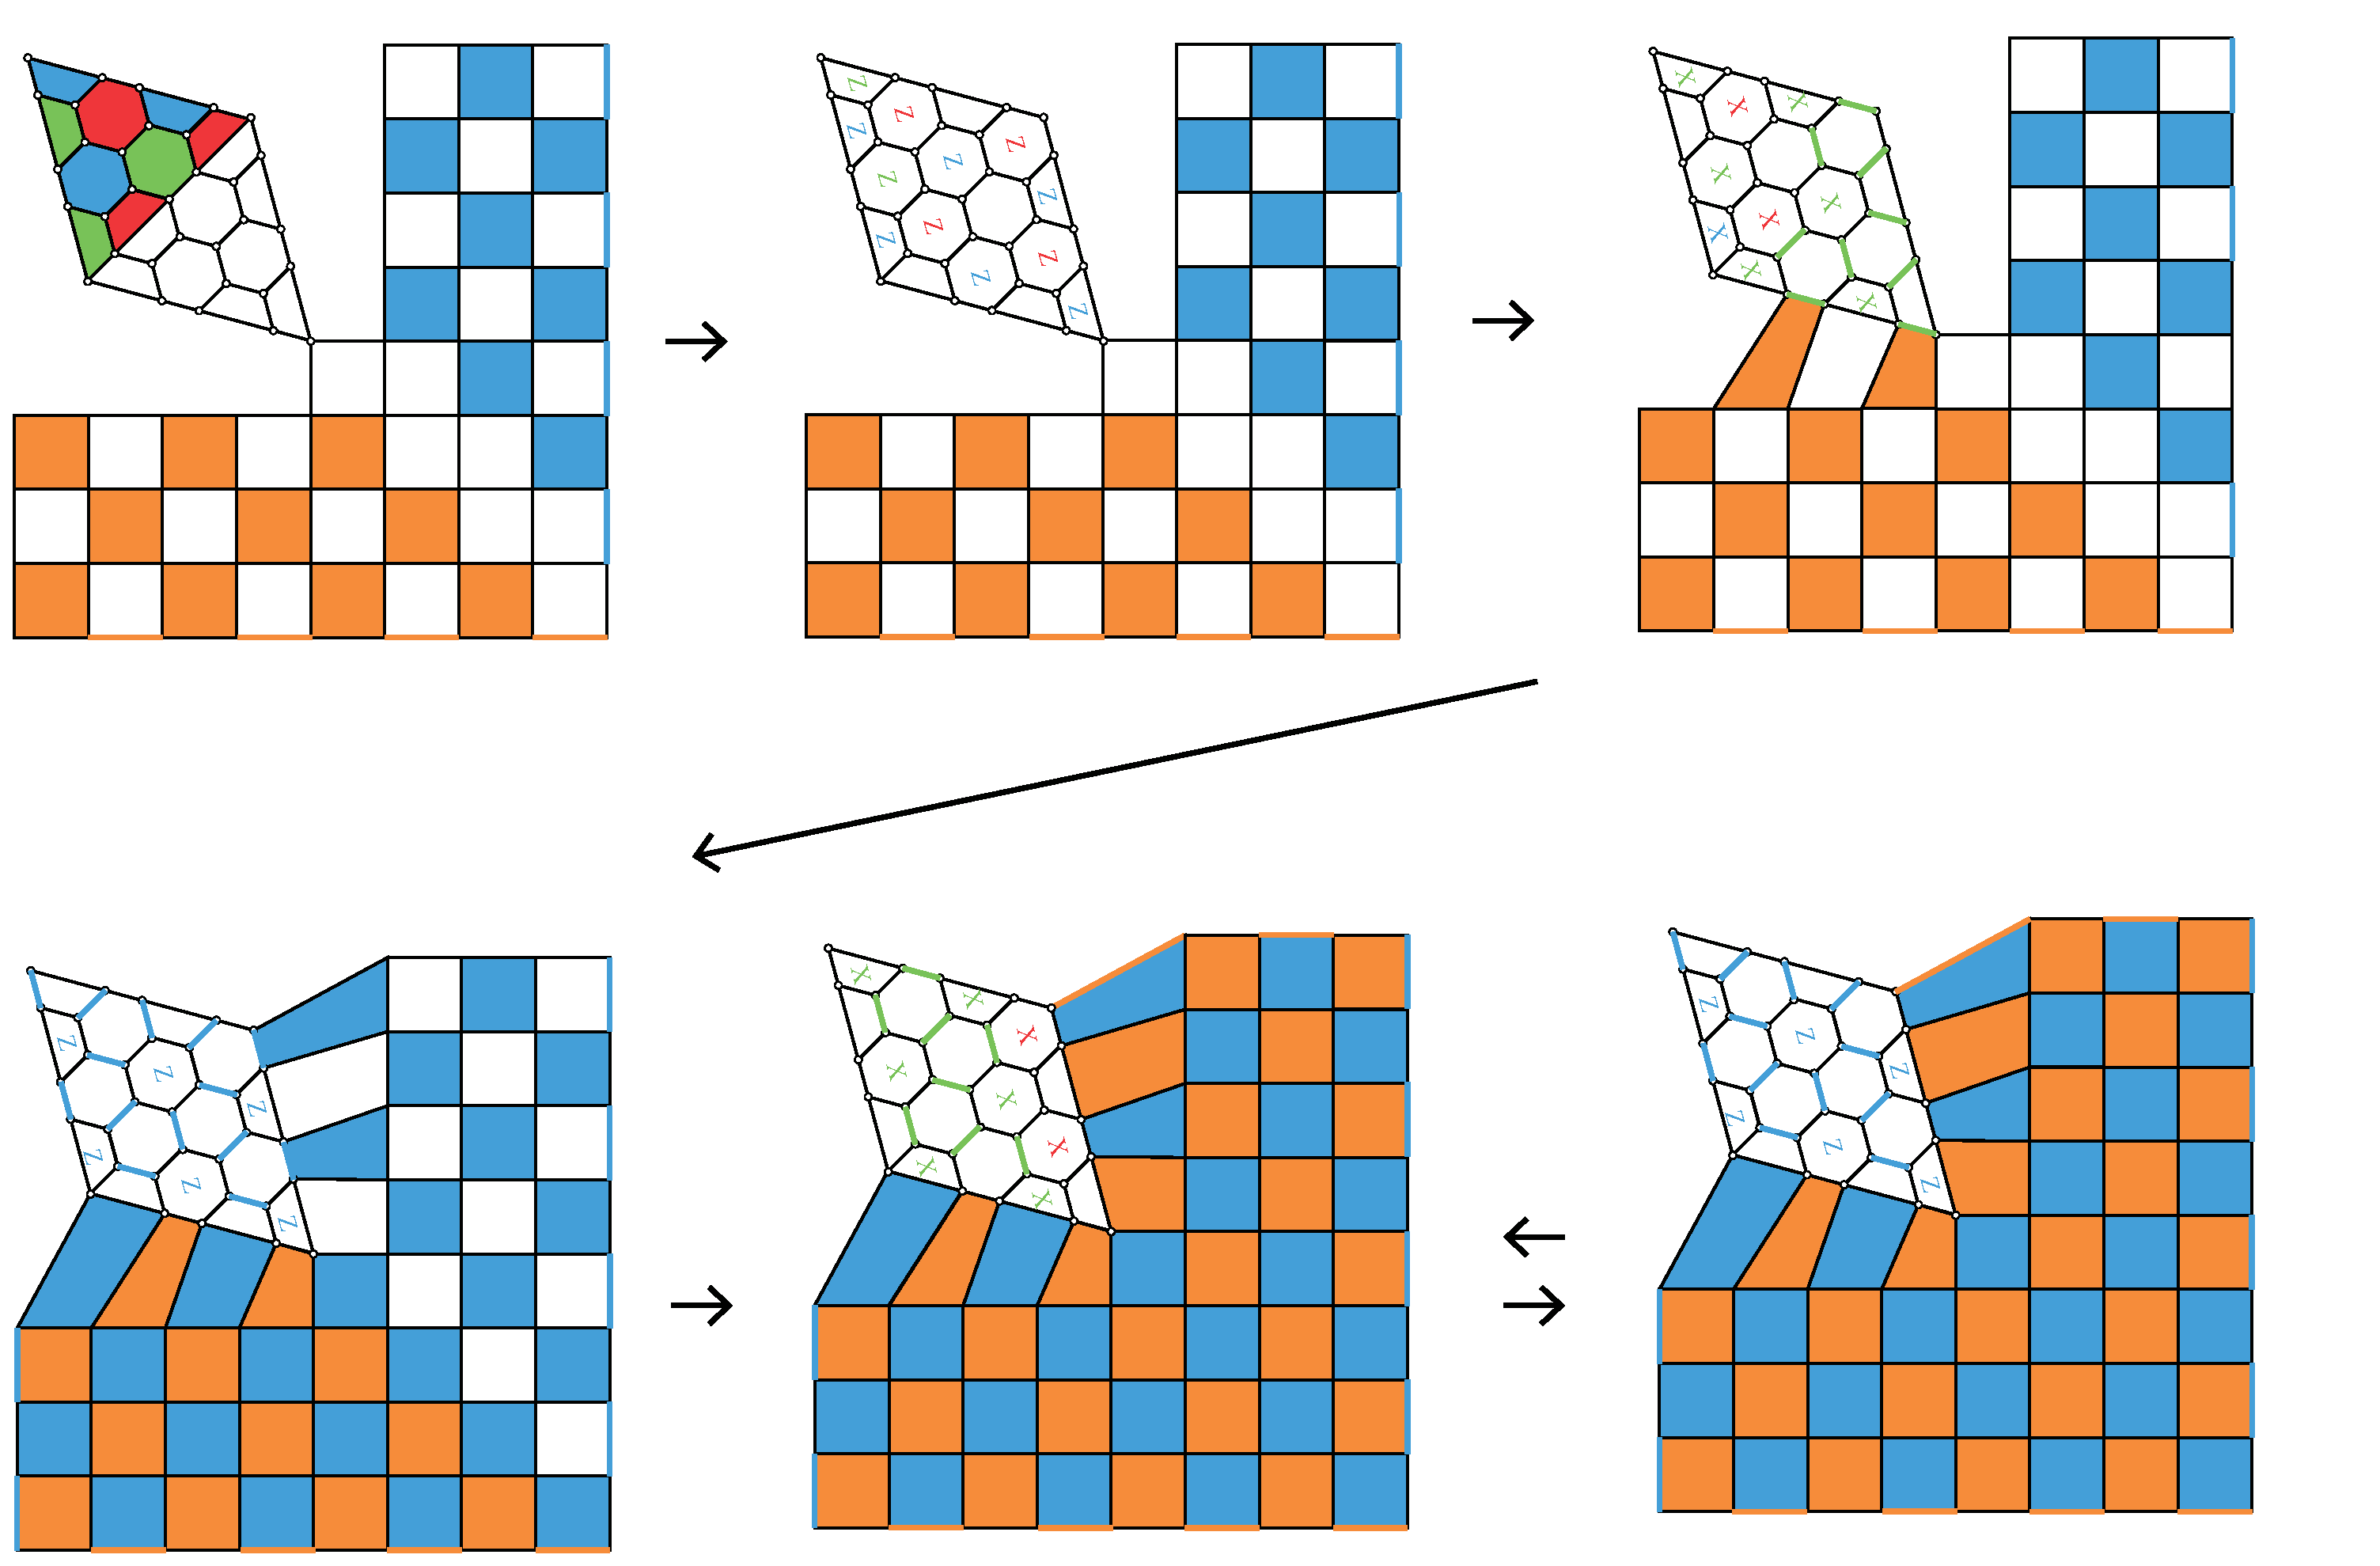
\includegraphics[scale=0.25]{figure/figure13.eps}
        \caption{ }
        \label{figure13}
    \end{figure}

    おそらくこの手順で実行すればエラーを見つけながらunfoldingと拡大を同時にできる。


}

\end{document}